\documentclass[a4paper, twoside]{report}

% Packages
\usepackage[a4paper]{geometry}				% a4 paper formatting
\usepackage[toc, page]{appendix}			% handles appendix
\usepackage[utf8]{inputenc}					% improves character compatability
\usepackage{textgreek}						% greek letters in text (references)
\usepackage{amsmath, amsfonts}				% math
\usepackage{xfrac}							% nicer fractions
\usepackage{algorithm, algcompatible}		% algorithm environment for pseudocode examples
\usepackage{graphicx, wrapfig}				% include pictures 
\usepackage{hyperref}						% active links in pdf
\usepackage{cleveref}						% automatic type of ref \cref{label}
\usepackage{tabularx}
\usepackage{csquotes}						% \enquote{text}

% 
% algorithm commands
\algnewcommand\INPUT{\item[\textbf{Input:}]}% 			% renames require to input
\algnewcommand\OUTPUT{\item[\textbf{Output:}]}%			% renames ensure to output
\algnewcommand\GIBBS{\item[\textbf{Gibbs Sampler:}]}%	% add gibbs sampler tag
\renewcommand{\algorithmiccomment}[1]{// #1}			% changes comments to //

% math sign commands
\newcommand\given[1][]{\:#1\vert\:}			% scalable conditional sign (\given)

% redefinition of caption. Bold highlight and regular text
\let\oldcaption\caption
\renewcommand\caption[2][]{\oldcaption[#1]{\textbf{#1:} #2}}


% import bib file
\usepackage[backend=bibtex8]{biblatex}		% bibliography package (bibtex)
\addbibresource{references.bib}



\begin{document}


\chapter*{Acknowledgements}
Tak alle sammen.
Også Ole

\chapter*{List of papers}
 
The dissertation is based on the following papers. They are presented in the order of publication.
\subsubsection{Paper 1}
EM Pedersen, E Agerbo, O Plana-Ripoll, J Grove, JW Dreier, KL Musliner, M Bækvad-Hansen, G Athanasiadis, A Schork, D Demontis, J Bybjerg-Grauholm, DM Hougaard, T Werge, M Nordentoft, O Mors, S Dalsgaard, J Christensen,  AD Børglum, PB Mortensen, JJ McGrath, F Privé, BJ Vilhjálmsson. Accounting for age-of-onset and family history improves power in genome-wide association studies. American Journal of Human Genetics, 109: 417-432.

\subsubsection{Paper 2}
EM Pedersen, E Agerbo, O Plana-Ripoll, J Steinbach, MD Krebs, DM Hougaard, T Werge, M Nordentoft, A Børglum,  KL Musliner, A Ganna, AJ Schork, PB Mortensen,  JJ McGrath,  F Privé, BJ Vilhjálmsson. ADuLT: An efficient and robust time-to-event GWAS. medRxiv, doi: https://doi.org/10.1101/2022.08.11.22278618 [Under review]

\subsubsection{Paper 3}
\textbf{\textit{Study 3:}} fGRS and fGRS multi trait [TBD - Under construction]
\mbox{}
\\

Besides these I have contributed to several other manuscripts that are not included in this dissertation. This includes the three published studies and one pre-print.

\begin{enumerate}
	\item MJ Witteveen, EM Pedersen, J Meijsen, MR Andersen, F Privé, D Speed, and BJ Vilhjálmsson. Publicly Available Privacy-preserving Benchmarks for Polygenic Prediction. bioRxiv, \url{https://doi.org/10.1101/2022.10.10.510645}
	\item T Wimberley, I Brikell, EM Pedersen, E Agerbo, BJ Vilhjálmsson, C Albiñana, F Privé, A Thapar, K Langley, L Riglin, M Simonsen, HS Nielsen, AD Børglum, M Nordentoft, PB Mortensen, S Dalsgaard. Early life injuries and the development of attention-deficit hyperactivity disorder.  Journal of Clinical Psychiatry, doi:\url{https://doi.org/10.4088/JCP.21m14033}.
	\item I Brikell, T Wimberley, C Albiñana, EM Pedersen, BJ Vilhjálmsson, E Agerbo, D Demontis, AD Børglum, A Schork, S LaBianca, T Werge, M Nordentoft, O Mors, D Hougaard, A Thapar, PB Mortensen, S Dalsgaard. Genetic, Clinical, and Sociodemographic Factors Associated With Stimulant Treatment Outcomes in ADHD.  American Journal of Psychiatry, doi:\url{https://doi.org/10.1176/appi.ajp.2020.20121686}.
	\item X Liu, T Munk-Olsen, C Albiñana, BJ Vilhjálmsson, E Pedersen, V Schlünssen, M Bækvad-Hansen, J Bybjerg-Grauholm, M Nordentoft, A Børglum, T Werge, D Hougaard, PB Mortensen, E Agerbo. Genetic liability to major depression and risk of childhood asthma. Brain Behavior and Immunity, doi: \url{https://doi.org/10.1016/j.bbi.2020.07.030}.
	
\end{enumerate}



% do I need a section with abbreviations ?
\tableofcontents
\newpage

\chapter{Introduction}

Over the couple of last decades, identifying genetic variants associated with diseases have been a major focus of research in human genetics; and for good reason. Identifying disease associated SNPs or genes provides insight into the genetic architecture of diseases and their aetiology. Ultimately, improved understanding of the diseases can lead to novel treatments and development of preventive measures. Although the field of genomics is still relatively young several promising discoveries have already been made. Some notable achievements include the development of genetic screening methods for disorders in the form of a polygenic risk score (PRS), identification of risk associated genes to target for drug development, as well as shining some light on the aetiology of complex and polygenic disorders. Individual genotypes may further inform diagnoses and help identify more effective treatment options through precision medicine. A principal driving factor behind these developments is the genome-wide association study (GWAS), which allows for the identification of SNPs or genes that are associated with a given phenotype. The associated SNPs can then be examined further with downstream analysis and their risk contributions can be aggregated to construct a PRS. Therefore, it is important to continue to improve GWAS methods and increase the statistical power in a GWAS setting, such that the developments can continue.

The two primary ways statistical power has been increased in a GWAS setting have been through sample size increases and methodological improvements. As individual-level genotypes cannot usually be shared, the sample size for most GWAS of disease phenotypes has been increased by meta-analysing GWAS from different cohorts. Several different methods for GWAS analyses have been proposed, including inverse-variance weighted meta-analysis\cite{willer2010metal}, and random effect meta-analyses to better capture genetic heterogeneity between cohorts\cite{han2011random}. The largest GWAS meta analysis performed so far is a GWAS of height where more than $ 5.4 $ million individuals\cite{yengo2022saturated}. Methodological improvements have also been made alongside the sample size increases. The improvements have mainly been in two directions, namely computational efficiency and more powerful GWAS models. As the field have evolved, knowledge about various complexities of GWAS have been discovered. This involves concepts such as in-sample relatedness (often called cryptic relatedness), different genetic ancestries, and population stratification. Initially, models such as linear regression was used, but it was poorly suited to account for such problems. Therefore models such as linear mixed models were suggested, as they are able to account for these problems. The BOLT-LMM\cite{loh2015efficient} software is an excellent example of an advancement that provided both computational efficiency and a more complex model. Prior to its publication, linear mixed models had a prohibitive computational cost, making them intractable for analysis of more than $ 100,000 $ individuals

While the sample sizes and methodological improvements are likely to continue, it is also worthwhile to consider related fields and their common practices. Taking inspiration from related fields and applying it in human genetics have already resulted in significant improvements to human genetics. Animal breeding share many similarities with human genetics and their computational tricks and commonly used models have already had an impact. For instance, some of the computational tricks employed by BOLT-LMM are inspired from animal breeding and the PRS are heavily inspired by the genetic breeding value employed in animal breeding\cite{loh2015efficient,wray2019complex,meuwissen2001prediction}. In epidemiology, animal breeding, and human genetics prior to the boom in genotyping, family history have been a strong and valuable predictor of many disorders \cite{guttmacher2004family,runeson2003family,collaborative2001familial,johns2001systematic}. One notable way family history has been used in human genetics is in the Framingham heart study\cite{kannel1990contribution,splansky2007third}, where it has been used to improve the risk assessment of heart disease.

Unfortunately, family history is not commonly available with genetic data in biobanks, which has limited the development of methods that can utilise family history in a GWAS setting. There are a small, but increasing number of biobanks that have some degree of family history linked to their genetic data. Some notable biobanks are UK biobank (UKBB) \cite{bycroft2018uk}, deCODE\cite{noauthor_2012-jh}, iPSYCH\cite{bybjerg2020ipsych2015}, and FinnGen\cite{Kurki2022-pt}. If family history is available, the coverage and source of the information is often not consistent across biobanks. In UKBB, only $ 12 $ disorders have family history information and it is acquired through questionnaires. iPSYCH has been linked to the Danish registers, which allows for the construction of complete family trees from $ 1969 $onwards with phenotypic information for each individual as well. FinnGen originates from Finland, who (like Denmark) is known for their detailed registers. However, FinnGen has limited family history linked to the genetic data due to privacy concerns. Only the parental cause of death has been allowed to be linked to the FinnGen genetic data so far, while far more information available in the Finnish registers. Even though the adoption of family history by biobanks has been limited, the family history methods that have been developed so far have shown a tremendous amount of potential. 

One of the first and most well-known family history methods that was developed is called genome-wide association study by proxy (GWAX). GWAX redefines the phenotype that is being analysed, and cases are individuals that are themselves affected by a disorder or have close family members that are. The researchers that proposed GWAX analysed Alzheimer's disease. Alzheimer's disease has a low prevalence among the UKBB participants, as many of them are not old enough to have been diagnosed with it yet, but many of their parents are. As a result, GWAX increased the number of considered cases. For low prevalence disorders, this has been shown to be useful when trying to identify genome-wide significant SNPs. Therefore, GWAX has been a success, provided a proof-of-concept and paved the way for other family history methods. GWAX itself has a limitation in that it loses power if the in-sample prevalence is high ($ >50\% $) for the GWAX phenotype. On top if this, it is a heuristic method and not based on any model. There have since been proposed a method called liability threshold model conditional on family history (LT-FH), which solves these two main limitations of GWAX. LT-FH is also the method that this dissertation have expanded further on to also allow for modelling of age of onset, sex, and cohort effects in the considered family members. The extension we developed is called LT-FH++.

To the best of our knowledge there is no other method available that is able to account for family history \textit{and} age of onset. All other methods seem to either model family history or age of onset, but never both. In terms of age-of-onset, the common first choice is some version of the Cox proportional hazards models (CoxPH). The time-to-event models that have been used in a GWAS setting so far are the CoxPH and the frailty model. The frailty model is a generalisation of the CoxPH model that also include a random effect that can model the in-sample relatedness (often called cryptic relatedness). Frailty models and mixed models share a lot of the same benefits, as they are both able to account for cryptic relatedness in a biobank. However, the adoption of frailty models has been slow. The slow adoption is likely due to several factors, where one of the main limitations is the computational complexity of these methods. Prior to the publication of the CoxPH model called SPACox in $ 2020 $, a CoxPH based GWAS was limited to $ <100.000 $ individuals due to computational cost\cite{bi2020fast}. However, other very computationally intensive models such as linear mixed models had been made computationally feasible for more than $ 400.000 $ individuals since $ 2015 $. Frailty models were similarly computationally intractable for more than $ 20.000 $ individuals up until $ 2022 $, where the method GATE was published. A computational trick that both SPACox and GATE utilise is a more efficient way of calculating p-values, such that more computationally intensive tests are no longer needed. SPACox and GATE use a saddle point approximation (SPA) that only require a cumulant generating function to efficiently estimate the p-value.

The dissertation has been focused on the development and applications of the LT-FH++ method, which is based on the age-dependent liability threshold model (ADuLT). If family history is included we will refer to the method as LT-FH++, and if only the index person is considered, we will refer to it as ADuLT. LT-FH++ combines many of the concepts from survival analysis and the CoxPH methods that have been developed for GWAS. It does this by extending the LT-FH method to also account for age of onset, sex, and cohort effects in the index and any included family members. Details on LT-FH and LT-FH++ are given in \cref{sec:methods:LTMs}. In short, LT-FH extends the classical liability threshold model proposed by Falconer to also incorporate family members, and LT-FH++ extends the model even further, such that age of onset can be modelled too. The LT-FH++ accounts for the age of onset by using a personalised threshold in the LTM, such that each threshold for determining case status depend on the age or age of onset, birth year, and sex. This means LT-FH++ utilises family history and a population representative cumulative incidence proportions (CIP). Through the CIPs it is possible to consider concepts such as censoring and stratification on sex and birth year, but in a liability threshold setup.

In other words, the family history methods have a clear benefit in that they are a drop-in replacement for any phenotype that is currently being used. If you consider Alzheimer's disease, then a GWAX phenotype will not require any fundamental changes to be made to an analysis plan, as the only change is the case-control status has been replaced by the GWAX phenotype. The same is true if a LT-FH phenotype is used, but with LT-FH there is no worry of any potential power loss, as it will always outperform GWAX and case-control phenotypes. This also holds true for LT-FH++ over LT-FH (and by extension GWAX). Since all of these phenotypes are drop-in replacements, it means that methodological advancements can be used immediately and will not require further implementation or modification to make them compatible with one another. An example of this could be a GWAS with a linear regression for a family history phenotype, being swapped to a linear mixed model one. No change would have to be made other than the choice of software to perform the GWAS. This means the family history methods builds on top of the methodological improvements that happen in parallel.

This is in contrast to the survival GWAS methods that have been proposed. They are all model specific implementations, such that a new model is will not be compatible with previous implementations. An example of this is SPACox and GATE. Both implementations invalidated any previously implemented CoxPH or frailty methods in a GWAS setting, as these allow for the analysis of far larger datasets. It also means that if a new, more complex model will be proposed at some point in the future that accounts for something yet to be determined, it will possibly invalidate both of these methods. While for the family history methods, they would immediately be able to utilise the new model and its implementation. LT-FH++ is therefore in a Goldilocks zone, as it is able to immediately utilise new methodological advancements, while preserving the survival analysis aspect and its inherent power increase.    

{\itshape
- Highlight relevance in relation to psychiatric disorders
}

TBD Text (raise points in the end of the introduction that can then be mentioned in the discussion / conclusion?)

%\chapter{Background}
%What is the background for this project? \textbf{first of all: Is this supposed to be the originally outlined project or what ended up happening in the end?}



\begin{enumerate}
\item How have researchers previously increased power in GWAS? (iirc, only through sample size and going from linear model to mixed models)
\item We wanted to increase power in GWAS without increasing the sample size. Attempts at this had already been made by including family history:
\begin{enumerate}
	\item GWAX, LT-FH
\end{enumerate}
\end{enumerate}



\chapter{Study aims}
The aims of the dissertation is to present an approach to account for both family history and time, as well as to improve the predictive value of family history in GWAS without increasing sample sizes. This was achieved by estimating a liability with a modified liability threshold model that depends on age-of-onset and family history. The thresholds used in the modified model are based on population representative cumulative incidence proportions stratified by sex and birth year. The following papers highlight different applications of the model.

\subsubsection{Paper 1: LT-FH++}
The first paper is the flagship paper of the dissertation. During the development of this paper, most of the implementation work was done such that estimating the desired liability was possible. The work resulted in the method titled LT-FH++, which is an extension of the previously published method LT-FH. LT-FH++ allows one to estimate a liability for an individual based on information such as age or age-of-onset, sex, birth year, and family history. This additional information can also be accounted for in each of the family members included, which was not possible with LT-FH. We found that the additional information did improve power, however in some cases it is only a modest improvement, since most of the power gain is driven by family history.

\subsubsection{Paper 2: ADuLT}
The second paper focused on the model underlying LT-FH++, called the age-dependent liability threshold (ADuLT) model, and its ability to increase power in GWAS compared to the more common Cox proportional hazards model. In this setting, the estimated liability depends on the same information as in the first paper, except we did not include family history and focused only on the age-of-onset aspect of the model. We only observed a notable difference between ADuLT and the Cox PH model when case ascertainment was present, but in such a case, the Cox PH was disproportionally affected and had a significantly lower power than ADuLT and even simple case-control linear regression.


\subsubsection{Paper 3: Family Liability}
The third paper is still in preparation and focuses on the predictive value of family history in the LT-FH++ model compared to the PRS and the conventional family history indicator. We estimate the liability in the LT-FH++ model, but excludes the index person's status and base the estimate solely on the family history. A multi-trait extension of the LT-FH++ model is also examined, where no disorder information is included on the index person. We found that the liability phenotype from LT-FH++ was significantly better than the binary family history variable, and the variance explained by the LT-FH++ phenotype was largely independent from the PRS. In the multi-trait case, the signal was still largely independent between the family history variables and the PRS, and the gap between The liability phenotype and the binary family history indicator was gone.


\chapter{Materials and methods}

\begin{enumerate}
	\item What data are we using and how are phenotypes defined?
		\begin{enumerate}
			\item Registers
			\begin{enumerate}
				\item Where do we get the diagnosis from? 
				\item How do we define disorders, age-of-onset, the study population
				\item How do we estimate the CIPs? Why do we need the population CIPs vs the in-sample prevalence/CIP.
			\end{enumerate}
			\item Genetic Data (describe iPSYCH and how it was sampled)
			\item Should I describe UKBB ?
		\end{enumerate}
	\item What methods are we using?
	\begin{enumerate}
		\item Were there any FH methods available when we started? (GWAX, LT-FH, other?)
		\item How do we simulate genotypes?
		\item The liability threshold model \& extensions
		\begin{enumerate}
			\item Describe the truncated normal distribution, how the covariance is determined, etc.
			\item How we estimate the liability (Gibbs sampler)
		\end{enumerate}
	\end{enumerate} 
	\item Should any genetics or GWAS be explained? e.g. SNPs, LD, etc... 
\end{enumerate}


\section{Data sources}

% danish registers
All projects in this dissertation are based on two types of information, register data and genotype data. The registers are used to define the study population, acquire phenotype information for individuals, and link family members. The genotype data is used to run a genome-wide association study (See section \textbf{TODO: ADD REF TO GWAS SECTION} for details). This dissertation aims to increase power of a GWAS without increasing the sample size of the genotyped data, but instead by utilising the additional information available from the registers. 
\textbf{TODO:ANY FIGURES THAT ARE GOOD AT ILLUSTRATING THE REGISTERS?}

\subsection{Danish registers}
The Danish registers provide the main source of phenotypic information and allow us to link individuals to their family members. The registers can be linked to one another through a unique 10-digit number assigned to every Dane and resident in Denmark since 1968.  

\subsubsection{The civil registration system}
The Danish civil registration system was established on 2 April 1968, and all persons living in Denmark were registered for administrative use. All registered individuals were given a 10-digit unique personal identification number, commonly referred to as the CPR-number. The CPR-number is used to link individuals across all registers. This register holds information on name, gender, date of birth, place of birth, citizenship, identity of parents, and is continually updated with information on vital status, place of residence and spouses. On 1 May 1972 all persons living in Greenland were also included into this register\cite{pedersen2011danish}. 

\subsubsection{The national patient register}
The Danish national patient register was established in 1977. Its contents has been expanded several times since it was created. Originally, it contained only information on patients admitted to somatic wards. In 1995, the register was expanded to also include outpatients, patients from emergency rooms, and patients from psychiatric wards. In 1994, the international classification of disease, version 10 (ICD-10) was adopted in Denmark, and prior to the adoption, ICD-8 was used\cite{lynge2011danish}. 


\subsubsection{The psychiatric central research register}
The psychiatric central research register has valid data from 1970 and onwards. At the beginning, the register contained information on every admission to a mental hospital and psychiatric department, where information such as dates of onset, end of treatment, and all diagnosis were recorded. In 1995, the register became an integrated part of the Danish national patient register and was expanded to also record information from psychiatric emergency room and outpatient treatment. Similar to the national patient register, ICD-10 codes were used after 1995, and ICD-8 were used before. Note that most mild and moderate affected individuals are treated by general practitioners or in private practices, in which case they are not recorded in this register.\cite{mors2011danish}


\subsection{Cumulative incidence proportions}
Another important usage for the registers is estimating population representative cumulative incidence proportions(CIPs) that are stratified by sex and birth year. These CIPs will form the basis of how we will account for age of onset. The CIPs have been estimated using the Aalen-Johansen estimator\cite{hansen2017estimating} with death and emigration as competing events. The Aalen-Johansen estimator estimates the survival function when competing events are present. Therefore, it should be used instead of the Kaplan-Meier estimator of the survival function if competing event are present. When stratified by sex and birth year, the CIPs can be interpreted as the proportion of individuals born in a given year and of a given sex who are diagnosed with a phenotype before a point in time $ t $. The data from the registers described above provide the basis for estimating these CIPs.
\textbf{TODO:ADD AN EXAMPLE CIP PLOT?}



\subsection{Genotype data}
This section covers the sources of genotype data used in this dissertation. There are two main sources, namely iPSYCH and UK biobank (UKBB). Here, we provide a brief overview for each of them. Notably, the iPSYCH cohort is a Danish biobank and has been linked to the previously mentioned registers. 

\subsubsection{The newborn screening biobank}
The Danish newborn screening biobank contains dried blood spot samples from nearly every newborn since 1982. The samples are taken from a heel prick a few days after birth and are stored at $ -20 $\textcelsius. Each year about $ 65,000 $ new samples are added, resulting in over $ 1.8 $ million samples in $ 2007 $. The purpose of the biobank is, among other things, to screen for various disease at birth. The samples are kept frozen for research purposes, and the dried blood spots provide the basis for the iPSYCH cohort. Accessing the dried blood spots for genotyping was granted after ethical approval from \textbf{TODO:LOOK WHERE APPROVAL CAME FROM} \textbf{MOVE TO THE REGISTRY SECTION?}  \cite{norgaard2007storage}.

\subsubsection{iPSYCH}
iPSYCH is short for the Lundbeck Foundation Integrative Psychiatric Research consortium, and it is the primary source of genotype data used in this dissertation. The benefit of a biobank such as iPSYCH is not the number of genotypes, instead its strength is due to the richness of the register information that it is linked to. All of the previously mentioned Danish registers have been linked to the genotypes, allowing for a very detailed set of phenotypes, as well as multiple information on each individual and their family members. The phenotypes of interest for the iPSYCH cohort are only psychiatric disorders, and they are ADHD, Autism, Anorexia, Bipolar disorder, Depression, and Schizophrenia\cite{pedersen2018ipsych2012}.

The iPSYCH cohort has been sampled in two rounds. The first round is called iPSYCH2012 and has $ 86,189 $ samples, while the second round, iPSYCH2015i, has $ 56,233 $ samples. The combined cohort is called iPSYCH2015 and has $ 141,265 $ unique samples. The population that iPSYCH2012 is nested within is defined as all singletons born in Denmark between the $ 1^{st} $ of May $ 1981 $ and the $ 31^{st} $ of December $ 2005 $, where the mother is known and the child is alive and living in Denmark by their first birthday. iPSYCH2015i extended the study population to individuals born between $ 1^{st} $ of May $ 1981 $ and $ 31^{st} $ of December $ 2008 $ with the same conditions. In total, $ 1,657,449 $ individuals satisfy this condition. For the first round of sampling, $ 30,000 $ samples were chosen at random, creating a population representative control group. For iPSYCH2015i another $ 21,000 $ were sampled for the control group. However, due to the random sampling $ 385 $ were chosen as controls for both iPSYCH2012 and iPSYCH2015i and another $ 2,958 $ individuals had at least one of the disorders iPSYCH focuses on, and would have been sampled either way. Any recorded case of the disorders of interest for iPSYCH would also be sampled. From the study population, all individuals with at least one of the focus disorders were sampled for iPSYCH2015 resulting in $ 93,608 $ samples, and $ 50,615 $ population controls\cite{pedersen2018ipsych2012,bybjerg2020ipsych2015}.

\subsubsection{UK biobank}

It is difficult to overstate the importance of the UK biobank's influence on the field of statistical genetics. Most importantly, UKBB is open access, meaning it is open to researchers from around the world, regardless of whether they are from academia, charity, or commercial sectors\cite{bycroft2018uk,biobank2015genotyping}. The biobank is also one of the largest of its kind with about $ 500,000 $ individuals, and it has rich phenotypic information from certain registers, such as cancer and death registers. Some electronic health records have also been linked to the participants, as well as questionnaires on socioeconomic and lifestyle factors. On top of this information, the participants also provided blood, urine, and saliva samples for proteomic and metabolomic analysis.
After imputation\cite{marchini2010genotype}, there are roughly $ 96 $ million genetic variants available. After filtering for genetic ancestry (see section \textbf{TODO: REFERENCE ANCESTRY SECTION}), a list of $ 409,728 $ individuals have been released with the data, as these individuals fall in a category with very similar ancestral backgrounds. Relatedness was not recorded during the recruitment process, so relatedness filtering had to be done with kinship coefficients for all pairs of participants. The relatedness analysis showed a larger than expected number of related pairs. The increase is likely due to sampling bias, as samples were taken from 22 recruitment centres across the UK, and close living relatives would be more likely to participate if one of them recommended it.
\textbf{TODO:Rewrite above section to focus more on family history and age of onset}



\section{Genome-wide association study}
%This section will briefly go over what a genome-wide association study (GWAS) is, some common considerations and models. A GWAS is usually performed on a single SNP at a time, rather than all SNPs at the same time. This is due to the computational cost of analysing data sets of the sizes that are usually present in biobanks and due to there being more SNPs than individuals. There are several potential models that can be used to analyse genotypes. One method is the Cochran-Armitage test \cite{cochran1954some,armitageTest}, which tests for independence in a $ 2\times 3 $ contingency table. However, this test is not able to incorporate covariates to account for, e.g. population stratification. A regression based method is usually preferred, as it allows for covariates to be included. One downside of using regression models is the assumption that the SNP effects will be additive, which is not the case in the Cochran-Armitage test. The genetic data for regression is usually coded as $ AA = 0 $, $ Aa = 1 $, and $ aa = 2 $, where $ A $ is the major allele and $ a $ is the minor allele\cite{zeng2015statistical}. When restricting to only additive genetic effects, there is no difference between logistic or linear regression and the Cochran-Armitage test. In short, the regression methods are preferred over the Cochran-Armitage test as covariates can be included and linear regression is preferred over logistic regression, since it is more computationally efficient and there is no difference between their power\cite{sikorska2013gwas,prive2019making,balding2006tutorial}.



This section will briefly go over what a genome-wide association study (GWAS) is, some common considerations, and models used. It will be split into sections that each cover an important topic for performing a GWAS, namely controlling type 1 errors, computational efficiency, and power improvement. At the end, we will also provide a non-exhaustive list of methodological advancements that excel in one or more of these topics. 

A GWAS is usually performed on a single SNP at a time, rather than all SNPs at the same time, meaning effect sizes are marginal instead of simultaneous. There are several potential models that can be used to analyse genotypes, and in the early days of GWAS the Cochran-Armitage test \cite{cochran1954some,armitageTest} was used \cite{balding2006tutorial}. The Cochran-Armitage test tests for independence in a $ 2\times 3 $ contingency table. However, this test is not able to incorporate covariates to account for important covariates such as population stratification. Therefore, regression based methods become popular, as they allow for covariates to be included. If a GWAS is performed with a regression, it implicitly assumed that the genetic effect from a given SNP will be additive, which is not the case for a Cochran-Armitage test. The implicit assumption follows from how the genetic data is coded for regression as $ AA = 0 $, $ Aa = 1 $, and $ aa = 2 $, where $ A $ is the major allele and $ a $ is the minor allele\cite{zeng2015statistical}. When restricting to only additive genetic effects, there is no difference between logistic or linear regression and the Cochran-Armitage test\textbf{TODO:REF}. 

In short, regression methods are preferred over the Cochran-Armitage test as covariates can be included and linear regression is preferred over logistic regression, since it is more computationally efficient and there is no difference between their power\cite{sikorska2013gwas,prive2019making,balding2006tutorial}.

First, the simplest and most common way to perform a GWAS will be introduced. Then each of the three important topics will be described and solutions to the problems will be presented.

\subsection{Linear regression GWAS} \label{sec:GWAS:LinReg}
The simplest and most computationally efficient way to test association between a SNP and an outcome, even when the outcome is binary, is with linear regression. If we have $ N $ individuals where we observe a set of $ M $ SNPs, then a linear regression GWAS of a single SNP can be described in the following way.

Let $ y $ denote the $ N\times1 $ vector of phenotypes for each individual, either binary or quantitative, $ X $ be the $ N \times (k+1) $ matrix containing $ k $ covariates and the intercept, $ G_j $ is a $ N\times 1 $ vector containing the $ j^{th} $ SNP, then the model is given by:

\begin{equation}\label{eq:baseGWAS}
y = \beta G_{j} +  X\gamma + \varepsilon.
\end{equation}
Where $ \beta $ denotes the genetic effect size, $ \gamma $ denotes a $ (k + 1) 
\times 1$ vector of coefficients for the intercept and covariates, $ 
\varepsilon $ is a $ N \times 1 $ vector of independent normally distributed 
noise. Going forward, we will assume that both $ y $ and $ G_j $ are scaled to 
have mean $ 0 $ and variance $ 1 $. The hypothesis being tested is $ H_0: \beta 
= 0 $ against $ H_A: \beta \neq 0 $. One of the most common ways to perform the 
test is with a Wald test $ Z = \hat{\beta}/\text{se}(\hat{\beta}) \sim N(0,1)$. 
\textbf{TODO: what is se(beta)} 



\subsubsection{Linear mixed model GWAS} 
A linear mixed model is an extension of a linear regression model. The linear mixed model adds a random effect to the model given in \cref{eq:baseGWAS}. With all other parameters being the same, we get


\begin{equation}\label{eq:baseMixedModelGWAS}
y = \beta G_{j} +  X\gamma + Zu + \varepsilon \qquad u \sim N(\mathbf{0}, \Sigma)
\end{equation}
The random term $ u $ and the noise $ \varepsilon $ are independent. Here $ Zu $ has an interpretation similar to $ X\gamma $, as $ 
Z $ is a design matrix for $ u $, but one that helps model the covariance structure. Then $ u $ is a random 
vector, and we can define the covariance structure of $ u $ by $ \Sigma $. In a GWAS setting, the covariance structure that one would 
like to model is some subset of SNPs. It can be achieved by letting $ Z = Z^{'}/\sqrt{M} $, where $ Z^{'} $ denotes the matrix 
with the desired subset of SNPs. Therefore, $ \Sigma $ will be a GRM calculated based on a preselected subset of SNPs. If 
we let $ K = ZZ^{T} $ denote the GRM on the subset of SNPs, we can express the covariance of the vector $ y $ in the following way

\begin{equation} \label{eq:MixedModelGWASCovariance}
cov(y) = \sigma_g^2K + \sigma^2_e I_N.
\end{equation}
Where $ \sigma^2_e $ is the environmental variance component, $ I_N $ is the $ N \times N $ dimensional identity matrix, $ \sigma_g^2 
$ is the genetic variance component, and $ K $ is the GRM on a subset of SNPs. With the choice of $ I_N $ for the environmental 
covariance structure, an independent environment is implicitly assumed for all individuals. Similarly, $ K $ allows individuals with a 
high correlation to be accounted for. The mixed model requires estimates of $ \sigma_e^2 $ and $ \sigma_g^2 $. Computationally, linear 
mixed models are far more intensive than linear regression, but the benefit of these models is their ability to boost power over 
simple linear regression. See \textbf{TODO: ref computational efficiency section} for details on computational and mathematical tricks 
that can speed up the computations.


\subsection{Controlling type-1 errors}
A common cause of type-1 errors (also called a false positive) is population structure. It is a term that covers several types of potential biases in a GWAS. These biases can result in spurious associations between SNPs and phenotypes, when there is no true association. The most common reasons for population structure in genotype data is due to \textit{population stratification} and \textit{related individuals}. Population stratification can have many causes. Every population will have some local structure, which may be problematic if not accounted for\textbf{REF?}. However, having two or more \textit{genetic ancestries} in the data in particular could severely bias a GWAS\textbf{REF?} and it is easy to account for. Regardless of the source of bias, they all result in the same underlying problem, namely artificial differences or similarities between a case and control group, which either creates a spurious association or masks a true association. \textbf{RFEFERENCE TO POP STRAT PROBLEMS?}
For example, if there is some kind of population structure in the data, common reasons are genetic ancestry or local variations within a population. A spurious association may occur if a subpopulation is particularly enriched with one type of variant and the rest of the population is not. Similarly, if the effect of a SNP in one genetic ancestry increases the risk, while it decreases the risk in a different genetic ancestry, then the effect of the given SNP would be hidden to us.

\subsubsection{Population stratification}
Within a population of individuals, it has been shown that there can be subpopulations where allele frequencies differ between subpopulations\cite{abdellaoui2013association,genome2014whole}. As mentioned above, it can cause artificial differences or similarities between the subpopulations when performing associations tests. One example of a spurious association driven by population stratification is the chopstick gene, which allegedly accounted for half of the variance in being able to eat with chopsticks \cite{marees2018tutorial,hamer2000beware}. A common and simple solution to account for local population stratification is to perform a PCA on the genotypes and including the first PCs as covariates in the association analysis \cite{price2006principal,price2010new,prive2020efficient}.

\begin{wrapfigure}{O}{10cm}
	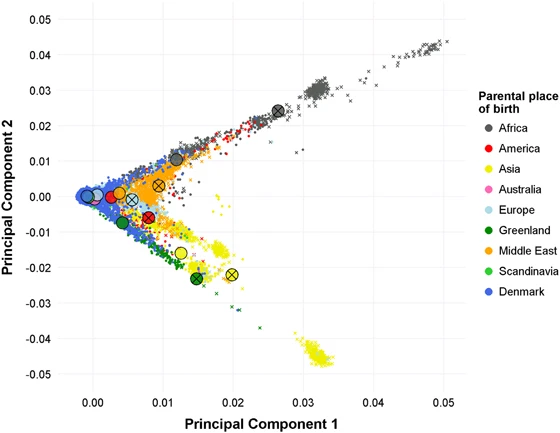
\includegraphics[width=10cm]{methods/iPSYCH_PCPlot.png}
	\caption[Scatter plot of the first two principal components of iPSYCH 
	participants coloured by parental country of birth]{The plot is provided without modification from the original paper describing 
	iPSYCH \cite{pedersen2018ipsych2012} \textbf{TODO:is it okay 
	to use a plot like this?}. The first two principal components have been 
	plotted for the iPSYCH participants and coloured according to the parent's 
	country of birth. The large circles indicate the mean values of a given 
	genetic ancestry group. The circles with a cross represent the individuals 
	where both parents are born in the region indicated by the colour, and no 
	cross means only one parent was.}
	\label{fig:ipsych_PCPlot}
\end{wrapfigure}


Population stratification can have many sources, and the above solution works if only local subpopulations are present in an otherwise homogeneous population. The problem arise if there are two or more genetic ancestries, as the PCs will not be able to properly account for such stratification. As a results, it seems prudent to highlight this particular cause of population stratification. Analysing different ancestries together in a GWAS is not commonly done. This is due to different ancestries having different minor allele frequencies for certain SNPs, altogether different variants on certain positions, etc.\cite{helgason2005icelandic}. Therefore, the most common way to deal with different ancestries in a genotyped data set is to identify a genetically homogenous subset and perform the association analysis in the homogeneous subpopulation. There have been methods proposed that can account for ancestry such as tractor\cite{atkinson2021tractor}, but they have not been widely adopted yet. 

A homogenous subpopulation can be identified by performing a PCA on all the 
available individuals and calculating a robust Mahalanobis distance on the 
first, e.g.\ 20 PCs, and removing anyone above a certain 
threshold\cite{prive2020efficient}. An illustration of the feasibility of 
identifying the genetic ancestry for the iPSYCH participants can be seen in 
\cref{fig:ipsych_PCPlot}.

\subsubsection{Relatedness}
Similar to population stratification, relatedness is a common cause of spurious associations. The mechanism behind why relatedness leads to these spurious associations is a little different. If related individuals are in the same analysis, then some individuals are more alike than one would expect if they were drawn at random. Due to this, deviations from the null distribution are likely to occur, not due to the SNP's effect, but rather the sampling. For a Wald test deviation could be expressed as a downwardly biased variance estimate, which leads to inflated test statistics, as the test statistics is the effect estimate divided by the standard error. \textbf{REF?}

There are two common ways to deal with relatedness in a GWAS setting. The first 
and simplest way is to identify the related individuals and removing them from 
the analysis. This is effective, but has the downside of reducing the sample 
size. The second and more involved way is to include the in-sample relatedness 
(sometimes also called cryptic relatedness) in the model being used for 
association. In a linear regression setting, the most common way to account for 
the in-sample relatedness is by using a linear mixed model, where a random 
effect that models the genotype correlation is added (see 
\cref{sec:GWAS:LinReg} 
for details). The random 
effect is able to account for the covariance structure of the individuals, 
which is how relatedness affects associations with higher than expected 
observations\cite{yu2006unified, kang2008efficient}. The in-sample relatedness 
is accounted for by having the covariance structure of the random effect follow 
the GRM.

If one decides to remove the related individuals instead, then there are several ways to identify the related individuals, with the 
two most common ways being the genetic relatedness matrix(GRM) and identity by descent(IBD)\textbf{TODO: REF TO HOW THESE ARE DONE?}. 
The GRM consists of the correlation between individual's genotypes, where a value of $ 1 $ means monozygotic twins, $ 0.5 $ is a 
parent-offspring relationship, etc.. If filtering is performed prior to the association test, the relatedness threshold is usually set 
to $ 2^{-2.5} \approx 0.177 $ when removing $ 2^{nd} $ degree relatives or closer, or $ 2^{-3.5} \approx 0.088 $ when removing $ 
3^{rd} $ degree relatives, etc. Filtering for relatedness with IBD is very similar to how it is done with the GRM, however the values 
are between $ 0 $ and $ 0.5 $ instead of $ 0 $ and $ 1 $ \textbf{TODO: are the values always between 0 and 0.5 for all IBD methods?}. 
To get the same level of relatedness filtering with IBD as one would get with the GRM, the thresholds should be shifted by a factor of 
$ 2^{-1} $ and will instead have thresholds $ 2^{-3.5} $ and $ 2^{-4.5} $, respectively. An IBD approach for identifying relatedness 
is provided by the KING software\cite{manichaikul2010robust}, and a GRM based approach is provided by the GCTA software 
\cite{yang2011gcta}. Both ways of estimating relatedness is also implemented in the PLINK 
software\cite{chang2015second,purcell2007plink}


\subsubsection{Multiple testing correction}
A GWAS consists of testing each available SNP for an association with the phenotype of interest. This means several million tests are often performed. A classical statical approach to hypothesis testing means a test has a significance threshold denoted by $ \alpha $, which is most commonly $ 5\% $. If the p-value is below $ \alpha $, the null hypothesis is rejected and the alternative hypothesis is accepted. Due to the p-values being uniformly distributed under the null hypothesis, we will expect to have $ (100\times \alpha) \%$ of the tests performed rejects the null hypothesis purely by chance. There are ways to account for this. The most common multiple testing correction method used in GWAS is the Bonferroni correction\textbf{REF}. As a motivation for the Bonferroni correction, let $ n $ independent tests be given, then the family-wide error rate $ \bar{\alpha} $, meaning the probability of seeing at least one false positive across all $ n $ tests, is given by

\begin{equation} \label{eq:bonferroni}
\bar{\alpha} = 1 - (1-\alpha)^n 
\end{equation}
$ \alpha$ is the per-test significance level. This leads to the Bonferroni correction $ \alpha_{bf} =  \alpha/n $. By comparing the repeated tests against $ \alpha_{bf} $ instead of $ \alpha $, the expected number of false positives will remain $ \alpha $ across all tests performed, thereby controlling the number of type-1 errors. In a GWAS setting, it is common to assume 1 million independent tests are performed \textbf{REF?}, which leads to a genome-wide significance threshold of $ 5 \times 10^{-8} $.



\subsubsection{Saddle point approximation}
\textbf{TODO: introduce SPA, as it is used by several methods}
\textbf{TODO: i do not want to derive anything. mention it can be used to estimate the CDF given a moment generating function is known and that is it ?}



\subsection{Computational efficiency}
This section will cover some of the common computational or mathematical tricks used to speed up GWAS. We will briefly describe how 
one can avoid estimating the effect sizes of covariates that have been included in the model and tricks on how to avoid 
inverting matrices. 



\subsubsection{Projecting covariates}
There is a computational cost involved in estimating the effects of the covariates. Therefore, the most efficient way to account for 
the covariates without directly calculating their effect in each regression is to project them out of the predictor and the response 
of interest in \cref{eq:baseGWAS} \cite{sikorska2013gwas}. For the sake of completeness, we will present how to regress out the 
covariates as they were presented by Sikorska et al.\cite{sikorska2013gwas}. 

Considering the residual sum of squares(RSS) for \cref{eq:baseGWAS}, we get 

\begin{align}
	RSS =& \left( y - \beta G_j - X\gamma \right)^T\left( y - \beta G_j - X\gamma \right) \\
	=& y^T y - 2\beta y^T G_j - 2y^TX\gamma - \beta^2 G_j^TG_j + 2\beta G_j^T X + \gamma^T X^T X \gamma.
\end{align}
Recall that $ X\gamma $ is a vector of dimension $ N \times 1 $, which means $ y^T X \gamma $ is an inner product and inner products are symmetric. Differentiating the residual sum of squares with respect to $ \beta $ and $ \gamma $ yields

\begin{align}
	\dfrac{\partial}{\partial \beta} (RSS) = -2y^TG + 2\beta G_j^TG_j + 2G_j^T X\gamma \\
	\dfrac{\partial}{\partial \gamma} (RSS)  = -2y^TX + 2\beta G^T_j X + 2X^TX\gamma 
\end{align}
Setting these expressions equal to $ 0 $, we get
\begin{align}
	G_j^T G_j \beta +  G_j^T X \gamma =  G_j^T y  \label{eq:covregress1}\\ 
	X^T G_j \beta + X^T X \gamma =  X^Ty \label{eq:covregress2}
\end{align}
This means the matrix notation of the least squares solution to \cref{eq:baseGWAS} is given by 
\begin{equation}
	\begin{pmatrix}
		G_j^T G_j & G_j^T X \\
		X^T G_j & X^T X
	\end{pmatrix}
	\begin{pmatrix}
		\hat{\beta} \\
		\hat{\gamma}
	\end{pmatrix} = 
	\begin{pmatrix}
		G_j^T y \\
		X^T y
	\end{pmatrix}.
\end{equation}
and we will let $ \hat{\beta} $ and $ \hat{\gamma} $ denote solutions to the least squares equations. However, we are interested in an expression that does not depend on the covariates. From here we isolate $ \hat{\gamma} $ in \cref{eq:covregress2} and get $ \hat{\gamma} = (X^TX)^{-1}(X^Ty - \hat{\beta} X^TG_j) $, which is then inserted in to \cref{eq:covregress1} 

\begin{equation}
	G^T_j y = G_j^TG_j + G_j^TX (X^TX)^{-1}(X^Ty - \hat{\beta} X^TG_j).
\end{equation}
By isolating terms related to $ y $ on the left hand side and term related to $ \hat{\beta} $ on the right hand side we get the following

\begin{equation} \label{eq:GWASprojection}
	G_j^T(y - X(X^TX)^{-1}X^Ty) = G_j^T(G_j - X(X^TX)^{-1}X^TG_j) \hat{\beta}.
\end{equation}
Recall that $ X(X^TX)^{-1}X^T $ denotes the projection onto the space spanned by the matrix $ X $. From here, we will introduce transformations given by 
\begin{align}
	y^\ast = y - X(X^TX)^{-1}X^Ty & & & G_j^{\ast} = G_j - X(X^TX)^{-1}X^TG_j.
\end{align}
The transformations remove the effect of the covariates in $ X $ from the response and predictor of interest. Using the properties of projections, \cref{eq:GWASprojection}, and the transformations, we find that 

\begin{equation}
	\left( G_j^{\ast} \right)^T G_j^{\ast} \hat{\beta} = G_j^T G_j^{\ast} \hat{\beta} \stackrel{\ref{eq:GWASprojection}}{=} G_j^T y^{\ast} = \left( G_j^{\ast} \right)^T y^{\ast}.
\end{equation}
The normal equation for systems of equations of the form $ Ax=b $ say that $ \hat{\beta} $ is a solution to a new univariate regression given by

\begin{align}\label{eq:univarGWAS}
	y^\ast = \hat{\beta} G_j^{\ast} + \varepsilon&   &\text{with simplified solution}&  &\hat{\beta} = \dfrac{\left( G_j^{\ast} \right)^T y^{\ast}}{\left( G_j^{\ast} \right)^T G^{\ast}}.
\end{align}
With the projection, the effect of the covariates have been removed from the outcome and the predictor, i.e. the phenotype and the genotype do \textit{not} depend on $ \gamma $ any more. Therefore, the calculations have been simplified and the calculations for the projection matrix only has to be performed once. Accounting for the covariate's effect in the phenotype also only has to be done once, the removal of the covariate's effect on the SNP has to be done for each SNP separately.
\textbf{TODO: Florian's thesis deals with speeding up computations even further, mention this too?}


\subsubsection{Avoiding inversions}

In this section, we will focus on ways of improving the computational efficiency of linear mixed models. First, a short introduction 
to which calculations are the most computationally intensive will be provided. Secondly, a way to circumvent the direct 
calculations will be provided. We will use the mixed model implementation in BOLT-LMM as an example. \textbf{TODO: does REGENIE and 
other methods use similar tricks ? if so, reference and highlight that here}

BOLT-LMM utilise a stochastic restricted maximum likelihood (REML) approach to estimate the variance components from 
\cref{eq:baseMixedModelGWAS}. The approach is called stochastic, since it utilise Monte Carlo sampling. The estimate acquired is a 
REML estimate, as all covariates have already been projected out of the phenotype vector, $ y $, the genotypes, $ G_j $, and the 
environment, $ \varepsilon $. This means degrees of freedom been reduced by $ C $, which is the rank of the design matrix $ X $. On 
top of this, all observations will now belong to an $ N-C $ dimensional subspace of $ \mathbb{R}^{N} $, and the distribution of the 
environmental term is now changed to $ \varepsilon \sim N(\mathbf{0}, \sigma_e^2 P)$, where $ P $ denotes the projection matrix on the 
space spanned by $ X $. Recall that a projection is symmetric and idempotent, hence only $ P $ is left in the covariance matrix of $ 
\varepsilon $. 

In this reduced setup, we will present how the variance components are estimated in an efficient manner under the infinitesimal model. 
First, we will reframe the problem in terms of a Bayesian setting where all of the covariates have been projected out. In the notation 
of \cref{eq:baseMixedModelGWAS}, we have

\begin{equation}\label{eq:bolt:infinitesimalModel}
y = Z\beta + \varepsilon, \qquad cov(y) = \sigma_g^2 K + \sigma_e^2 P
\end{equation}
where each SNP's effect has the prior $ \beta_j \sim N(0, \sigma_j^2)$ with $\sigma_j^2 = \sigma_g^2 / M $. The \textit{stochastic} 
REML then simulates observations under the model in \cref{eq:bolt:infinitesimalModel} and attempts to find a solution to an 
equivalent problem. With a slight abuse of notation of $ \lVert \varepsilon \rVert^2$ and  $ \lVert \beta \rVert^2$, we can phrase the 
alternative problem that we will solve as

\begin{equation} \label{eq:bolt:AlternativeMMEProblem}
E\left[ \sum \hat{\varepsilon}^2_{rand} \right] = \sum \hat{\varepsilon}^2_{data}, \qquad E\left[ \sum \hat{\beta}^2_{rand} \right] = 
\sum \hat{\beta}^2_{data}.
\end{equation}
Here $ \hat{\beta}^2_{data} $ and $ \hat{\varepsilon}^2_{data} $ are the BLUP estimates in \cref{eq:bolt:infinitesimalModel}. The 
terms in the expectation are $ \hat{\beta}^2_{rand} $ and $ \hat{\varepsilon}^2_{rand} $ and they are simulated values under the same 
model, but with a known and fixed $ \sigma_g^2 $ and $ \sigma_e^2 $. The simulated values are given by

\begin{equation} \label{eq:bolt:AlternativeMMEobs}
y_{rand} = Z \beta_{rand} + \varepsilon_{rand}, \qquad \beta_{rand,j} \sim N(0, \sigma_j^2),  \qquad \varepsilon_{rand,j} \sim N(0, 
\sigma_e^2).
\end{equation} 
Hence, the left hand side of \cref{eq:bolt:AlternativeMMEProblem} can be estimated by samples generated from 
\cref{eq:bolt:AlternativeMMEobs} with fixed and known variance components and the right hand side can be estimated with a BLUP 
estimator. This setup allows for iteratively calculating the BLUP estimates and estimating the variance components. We will outline 
how this iterative scheme is performed now. First, we will assume that we have $ \sigma_g^2 $ and $ \sigma_e^2 $ known and fixed. 
Then, we will define the following 

\begin{align}
	\delta := \dfrac{\sigma_e^2}{\sigma_g^2}, \qquad H := K + \delta I_N.
\end{align}
From here, the BLUP estimates are given by
\begin{align} \label{eq:bolt:iteratativeBLUP}
	\hat{\beta} = \dfrac{1}{M}Z^T H^{-1} y,  \qquad  \hat{e} = \delta H^{-1}y
\end{align}
Note that the BLUP estimates are constant for a fixed $ \delta $. With this, we can calculate the BLUP estimates. Next, we need a way 
to find estimates of the variance components, $ \sigma_g^2 $ and $ \sigma_e^2 $. We will rephrase \cref{eq:bolt:AlternativeMMEProblem} 
as a single equation that depends on $ \delta $ with 

\begin{equation}
\dfrac
{E\left[ \sum \hat{\beta}^2_{rand} \right]}
{E\left[ \sum \hat{\varepsilon}^2_{rand} \right]}
 =
\dfrac
{\sum \hat{\beta}^2_{data}}
{\sum \hat{\varepsilon}^2_{data}}.
\end{equation}
where we can scale $ \sigma_g^2 $ such that it matches the observed data. From here, we can get $ 1 $ on the left hand side of the 
rephrase equation above, and take the logarithm on both sides to get

\begin{equation}\label{eq:bolt:iterativeRatio}
f_{reml}(\log(\delta)) 
:= \log 
\left(
\dfrac
{
E\left[ \sum \hat{\varepsilon}^2_{rand} \right]	
\sum \hat{\beta}^2_{data}
}
{
\sum \hat{\varepsilon}^2_{data}
E\left[ \sum \hat{\beta}^2_{rand} \right]
}
\right).
\end{equation}
As a result, we have to find a value of $ \delta $ which satisfy $ f_{reml}(\log(\delta)) = 0$. We will not elaborate on the details 
of how this is done, but it involves using the secant method and a sampling strategy similar to the one used above for the BLUP 
estimate. In summary, estimating the variance components in a mixed model, as presented in BOLT-LMM, means calculating the BLUP 
estimates in \cref{eq:bolt:iterativeBLUP} and finding $ \delta $ that solves \cref{eq:bolt:iterativeRatio}. However, the calculations 
needed to perform the iterative scheme require inverting a matrix. Matrix inversion is computationally expensive and has computational 
complexity of $ O(N^3) $ if calculated naively \textbf{TODO:ref?}. Other strategies have been suggested, which allows for a 
computational complexity of $ O(NM^2) $ or $ O(N^2M) $ \textbf{TODO:ref}. The strategy employed in BOLT-LMM has a computational 
complexity of $ O(NM) $. 

The variance of the phenotype, as seen in \cref{eq:MixedModelGWASCovariance} or in the iterative scheme as 
\cref{eq:bolt:iterativeBLUP} will have to be inverted, if calculated naively. We can efficiently perform calculations of the form $ 
H^{-1}y $ and circumvent the inversion by not directly forming $ H $, but instead considering its terms, $ ZZ^T / M$ and $ \delta I_N 
$. If we multiply with some vector, $ q $, from the right, then it is only the GRM term that is computationally expensive. However, we 
can express it in the following way

\begin{equation}
ZZ^T q = \sum_i \left( Z_i Z_i^T\right) q = \sum_i  Z_i \left(Z_i^T q\right) 
\end{equation}
The first equation expresses $ Z Z^T $ as the sum of the outer products of columns of $ Z $ and the second as a sum of vectors times a 
scalar, where the scalar is the result of an inner product between the $ i^{th} $ column of $ Z $ and the given vector $ q $. This 
reformation of the product $ Z Z^T q$ has computational complexity $ O(NM) $.

\textbf{TODO: i am not sure, but it almost seem like it is suggested that $ (A + B)^{-1} = A^{-1} + B^{-1} $, which i do not think 
holds generally. they specifically say in the suppNotes that they do not form H and only consider the terms individually and multiply 
from the right with a vector.}


%%%

%Note, BOLT-LMM utilise several tricks and it is beyond the scope of this dissertation to go over all of them in detail. We will 
%mainly 
%consider how the variance components are estimated, as an integral part of using a linear mixed model is estimating the variance 
%components. The linear mixed model used by BOLT-LMM has a variance given by

%\begin{equation}
%var(y) = \sigma_g^2 \dfrac{G^TG}{M} + \sigma_e^2 P
%\end{equation}
%where $ \sigma_g^2 $ and $ \sigma_e^2 $ are the genetic and environmental variance components respectively. In particular, $ G^TG/M $ 
%is the GRM and models the covariance structure present in the genotypes, and $ P $ is a projection on a covariance spanned subspace 
%(See \textbf{TODO: reference the projection section}). The variance components are estimated by a Monte Carlo restricted maximum 
%likelihood (REML) approach\textbf{REF}. Note, the approach becomes REML due to the projection. Following the Monto Carlo REML 
%approach 
%touches on several computational challenges, but one of the most important ones is inverting a large matrix. Notably, they rephrase 
%the problem of estimating the variance components, and it therefore boils down to solving a system of equations that depend on the 
%following values.
%
%\begin{align}
%	\delta = \dfrac{\sigma_e^2}{\sigma_g^2} & & & H = \dfrac{G^T G}{M} + \delta I_N
%\end{align}
%From here, the BLUP estimates are given by
%\begin{align}
%\hat{\beta} = \dfrac{G^T H^{-1}}{M} y & & & \hat{e} = \delta H^{-1}y
%\end{align}
%With a fixed $ \delta $, the BLUP estimates are constant. 
%
%
%In particular, this means calculating $ H^{-1}$, which requires inverting a $ N \times N $ matrix. Naive matrix inversion requires $ 
%O(N^3) $ operations, which can be restrictive for large $ N $. Computational tricks can be applied, which lower the computational 
%complexity to $ O(NM^2) $ or $ O(N^2M) $. The BOLT-LMM solves this with conjugate gradient iteration, which has computational 
%complexity $ O(NM) $.\textbf{REF}
%More precisely, it is possible to calculate expression of the form $ H^{-1}y $ with only products of $ H $ with some vector. 
%\textbf{REF} These calculations only work because $ H $ is positive semidefinite.
%
%\textbf{TODO: should I give some details on the conjugate gradient iteration used?}
%
% \cite{legarra2008computing}: conjugate gradient iteraton paper

%BOLT-LMM utilise a mixed linear model with a Gaussian mixture prior, which allows for a non-infinitesimal model. 
%BOLT steps
%(1a) estimation of variance parameters; 
%circumvents spectral decomposition with stochastic approximation algorithm instead. it requires finding a solution to a linear systems of mixed-model equations instead, which is done by conjugate gradient iteration.
%(1b) computation of infinitesimal mixed-model association statistics (BOLT-LMM-inf); 
%circumvents spectral decomposition by introducing a new retrospective mixed-model association statistic similar to GRAMMAR-Gamma10 and MASTOR23, which we compute—up to a calibration constant—using only the solutions to linear systems of equations. We estimate the calibration constant by computing the new statistic and comparing it to the standard prospective mixed-model statistic at a random subset of SNPs; this step can likewise be accomplished efficiently using conjugate gradient iteration. This procedure is similar in spirit to GRAMMAR-Gamma calibration but requires only O(MN) time iterations.
%(2a) estimation of Gaussian mixture-model parameters; 
%
%(2b) computation of Gaussian mixture-model association statistics (BOLT-LMM)

\subsection{Model driven power improvement}
\textbf{TODO: refine phenotype reduces residual var -> increases power}

Increasing power to detect the true associations has been another primary focus of GWAS method developments. The leap from linear regression to a linear mixed model is expected to provide a power increase \textbf{REF?}. The increase comes from modelling the covariance structure present in the data, which is not possible for linear regression. As the covariance structure is modelled, it is no longer necessary to remove individuals due to relatedness or population stratification. This has the additional benefit that the sample size increase, which in turn increases power. 

Another source of power improvement is accounting for the effect of other SNPs. When one accounts for other SNPs in this manner, it essentially means a reduction in the residual variance of the phenotype, which is also why it has been referred to as \textit{denoising} the phenotype\textbf{REF}. Reducing the residual variance of the phenotype has proven to be an effect way to increase power in a GWAS, and we will briefly present how it can be done. Again, we will use BOLT-LMM as an example.

In BOLT-LMM, they utilise an infinitesimal model and a Bayesian model with mixture Gaussian priors. This mixture model allows for a non-infinitesimal model to be used, as some SNPs will be set to $ 0 $ and the variance for groups of SNPs can vary.  In a linear mixed model setup, as seen in \textbf{REF: to mixed model section} and with the covariance of $ y $ given as $V = \sigma_g^2G^TG/M + \sigma_e^2I_N $, the test statistic is given by

\begin{equation}\label{eq:boltLMMchisq}
\chi^2_{LMM} = \dfrac{(G_j^TV^{-1}y)^2}{G_j^TV^{-1}G_j}
\end{equation}
with $ \sigma_g^2 $ and $ \sigma_e^2 $ estimates under the null hypothesis $ H_0: \beta = 0 $. However, performing a test in this way means accounting for the same SNPs more than once, as the SNP of interest will also be present in the GRM. We can avoid it by removing the chromosome that the $ j^{th} $ SNP belongs to from the GRM calculations. This is called leave-one-chromosome-out (LOCO). We will denote the LOCO GRM as $ V_{LOCO} = (G_{LOCO})^TG_{LOCO}/M_{LOCO}$, where $ G_{LOCO} $ is the SNP that remain after removing the $ j^{th} $ SNP's chromosome and $ M_{LOCO} $ is the number of SNPs after removing the same chromosome. We get the LOCO test statistic to be

\begin{equation}\label{eq:boltLMMchisqLOCO}
\chi^2_{LOCO} = \dfrac{(G_j^TV_{LOCO}^{-1}y)^2}{G_j^TV_{LOCO}^{-1}G_j}
\end{equation}
Notably, this means calculating a $ V_{LOCO} $ for each chromosome. The BOLT-LMM infinitesimal model has a test statistic that is given by

\begin{align}\label{eq:boltLMMinfchisq}
\chi^2_{BOLT-INF} = \dfrac{(G_j^TV_{LOCO}^{-1}y)^2}{c_{inf}} & &c_{inf} = \dfrac{\text{mean}((G_j^TV_{LOCO}^{-1}y)^2)}{\text{mean}(\chi^2_{LOCO})}
\end{align}
Where $ c_{inf} $ is chosen such that $ \text{mean}(\chi^2_{BOLT-INF}) = \text{mean}(\chi^2_{LOCO})$. The constant $ c_{inf} is $ estimated from $ 30 $ pseudorandom SNPs.

When introducing the Gaussian mixture prior, they generalise the test statistic as

\begin{equation}\label{eq:boltMixturePriorTestChisq}
\chi^2_{BOLT-LMM} = \dfrac{\left( G_j^T y_{residual}\right)^2}{c}
\end{equation}
where $ y_{residual} $ is a residual phenotype vector obtained after fitting a Gaussian mixture extension of the standard LMM. The LMM model to fit the phenotype is still using LOCO, but to ease notation, the notation has been suppressed. The calibration factor $ c $ is chosen such that the intercept of $ \chi^2_{BOLT-LMM} $ with the LD score regression model\textbf{REF LDSC} matches the intercept of the properly calibrated $ \chi^2_{BOLT-INF} $.

The test statistic for the non-infinitesimal model require calculating the residualised phenotype $ y_{residual} $. Next we will describe how those are obtained. Under a Bayesian framework, the null model associated with \cref{eq:boltLMMchisqLOCO} is given as

\begin{equation}\label{eq:boltBayesLMMWithPrior}
y = G_{LOCO} \beta_{LOCO} + \varepsilon \qquad \beta_j \sim N(0, \sigma^2_g /M_{LOCO}), \qquad \varepsilon \sim N(\mathbf{0},\sigma_e^2I_N)
\end{equation}
Note that the model is infinitesimal as all SNPs $ \beta_j $ follow the same distribution. The generalisation to a Gaussian mixture prior means replacing the prior for $ \beta_j $ with 

\begin{equation}
\beta_j \sim
\begin{cases}
N(0, \sigma^2_{g1}) & \text{with probability } p \\
N(0, \sigma^2_{g2}) & \text{with probability } 1-p
\end{cases}
\end{equation}
This prior is sometimes called a spike-and-slab prior, since one of the variances $ \sigma^2_{g1} $ or $  \sigma^2_{g2} $ may be very large while the other may be very small. This results in two normal distributions, one very concentrated around $ 0 $, and another that allows for large variations in effect sizes. If illustrated, this looks like a spike around $ 0 $, and a slab covering a large area, hence the name.

The effect sizes, $ \beta_j $, are estimated from \cref{eq:boltBayesLMMWithPrior}, and the residualised phenotype under the Gaussian mixture prior vector is calculated as

\begin{equation}
y_{residual} = y - G_{LOCO}\beta_{LOCO}
\end{equation}
The residualised pheotype vector, $ y_{residual} $, is then used in \cref{eq:boltMixturePriorTestChisq}. By using the mixture prior, BOLT-LMM has a $ 25\% $ increase in effective sample size compared to the infinitesimal model.
\textbf{TODO: Should I make a summary paragraph?}


\subsection{Notable methodological advancements}
This section provides a non-exhaustive list of methodological advances proposed for GWAS. The list aims to highlight key advances that have been made by either providing computational feasibility for a certain type of analysis, use of a more complex model, or both. Notable GWAS methods are presented in \cref{table:GWASoverview}. 

\begin{table}[h]
	\centering
	\begin{tabularx}{\textwidth}{l X l}
		\hline
		Software	&	Notable advancement		&	Model \\
		\hline
		PLINK\cite{chang2015second,purcell2007plink}	&
		Highly scalable linear and logistic regression \& Data management and standardized a binary storage format	&
		Linear \& logistic regression	\\
		BOLT\cite{loh2015efficient}	&
		Efficient linear mixed model for UKBB sized data that accounts for cryptic relatedness \& increases power	&
		Linear mixed model	\\
		SPACox\cite{bi2020fast}	&	
		Saddle point approximation based proportional hazards model for UKBB sized data &
		Cox proportional hazards \\
		GATE\cite{dey2022efficient}	&
		Saddle point approximation based frailty model for UKBB sized data	&
		Frailty model \\
		\hline
	\end{tabularx}
	\caption{Overview of notable GWAS methods}
	\label{table:GWASoverview}
\end{table}
Other methods that are based on the saddle point approximation (SPA)\cite{daniels1954saddlepoint,kuonen1999miscellanea} have been proposed by methods such as SAIGE\cite{zhou2018efficiently} and REGENIE\cite{mbatchou2021computationally}. One of the advantages of using SPA is that it provides good control of Type 1 error, even for unbalanced case-control phenotypes. While BOLT-LMM provided an efficient implementation for linear mixed models, further study of the software have revealed that it suffers from inflated test statistics when case-control ratio is $ 1:50 $ or higher. SPA-based methods do not suffer from inflation in such cases\cite{mbatchou2021computationally}.








\chapter{Results}



perhaps structure the results section by paper in this way:

\begin{enumerate}
	\item LT-FH++: highlight Mortality and ADHD. It shows the importance of including family history and age-of-onset to increase power, but also shows that it is not the end all be all.
	\begin{enumerate}
		\item Mortality GWAS - large power increase
		\item ADHD GWAS - almost no power increase
	\end{enumerate}
	\item ADuLT: when only looking at age-of-onset, cox PH models are probably not the best model to use. ADuLT is \textit{never} the worst model, but also not always the best. The most robust method is ADuLT, since power is always best or close to the best.
	\begin{enumerate}
		\item simulation results with downsampling
		\item ADHD GWAS results
	\end{enumerate}
	\item fGRS: the predictive performance of the liabilities compared to binary variables.
	\begin{enumerate}
		\item single trait performance
		\item multi trait performance 
		\item cross ancestry performance
	\end{enumerate}	
\item Do I need a section combining the results into a larger picture somehow here ? or is it meant to go in the discussion?
\end{enumerate}


This section will summarise the results of the papers the dissertation is based on.

\section{Paper 1 - LT-FH++}
The first paper proposed the method LT-FH++, which is an extension of the previously proposed LT-FH method by Hujoel et al\cite{hujoel2020liability}. The notable difference between LT-FH and LT-FH++ is the ability to account for age of onset for cases or age for controls, sex, and birth year, as well as the same information in the included family members. The LT-FH method does not consider sex or age in parents, meaning they have the same thresholds. It also uses the same threshold for the index person and siblings and does not distinguish on age or sex differences. LT-FH++ is also able to account for siblings individually rather than considering the number of siblings and an \enquote{\textit{at least one affected sibling}} indicator. This way of coding siblings in LT-FH is likely due to the way sibling information is coded in the UKBB, which was the main application of the LT-FH paper. Considerable changes have also been made to the sampling strategy to allow for the increased flexibility in the family and the use of personalised thresholds to be scalable to millions of individuals.  The changes LT-FH++ proposed increased the number of unique configurations considerably, as each individual now has a unique set of family members and thresholds. The sampling strategy used for LT-FH would be computationally intractable for LT-FH++, since LT-FH only needed to estimate a liability for a handful of configurations.


\subsection{Simulation results}
We performed simulations to assess the power and false discovery rate of LT-FH++ against LT-FH and a case-control status to detect causal SNPs in a linear regression GWAS. The simulations are based on simulated genotypes, where we simulated a pair of parents and one offspring with no siblings. We used parameters similar to the ones used in the LT-FH paper to ensure compatibility between findings. The simulated genotypes had a heritability on the liability scale of $ h^2 = 0.5 $, a population prevalence of $ 5\% $. Unlike in the LT-FH paper, we used a higher prevalence in one of the simulated sexes, but the combined prevalence would still be $ 5\% $. The case ratio was $ 1{\,:\,}4 $ between sexes, and it was also present in the parents. We also considered a population prevalence of $ 10\% $, but those results are not shown here. The genotypes consisted of $ 100,000 $ individuals, each with $ 100,000 $ independent SNPs where $ 1000 $ SNPs were causal, i.e.\ they had a simulated effect size different from $ 0 $. The simulation results shown in \cref{fig:LTFHppSimulationResults} are based on $ 10 $ replications of each simulation scenario. Case ascertainment is common in biobanks, which means there is a higher (or lower) prevalence of a phenotype of interest in the biobank compared to the rest of the population. We emulated case ascertainment in the simulations by downsampling the entire population until we had a subpopulation with $ 10,000 $ individuals with the same number of cases and controls.

\begin{figure}[h]
	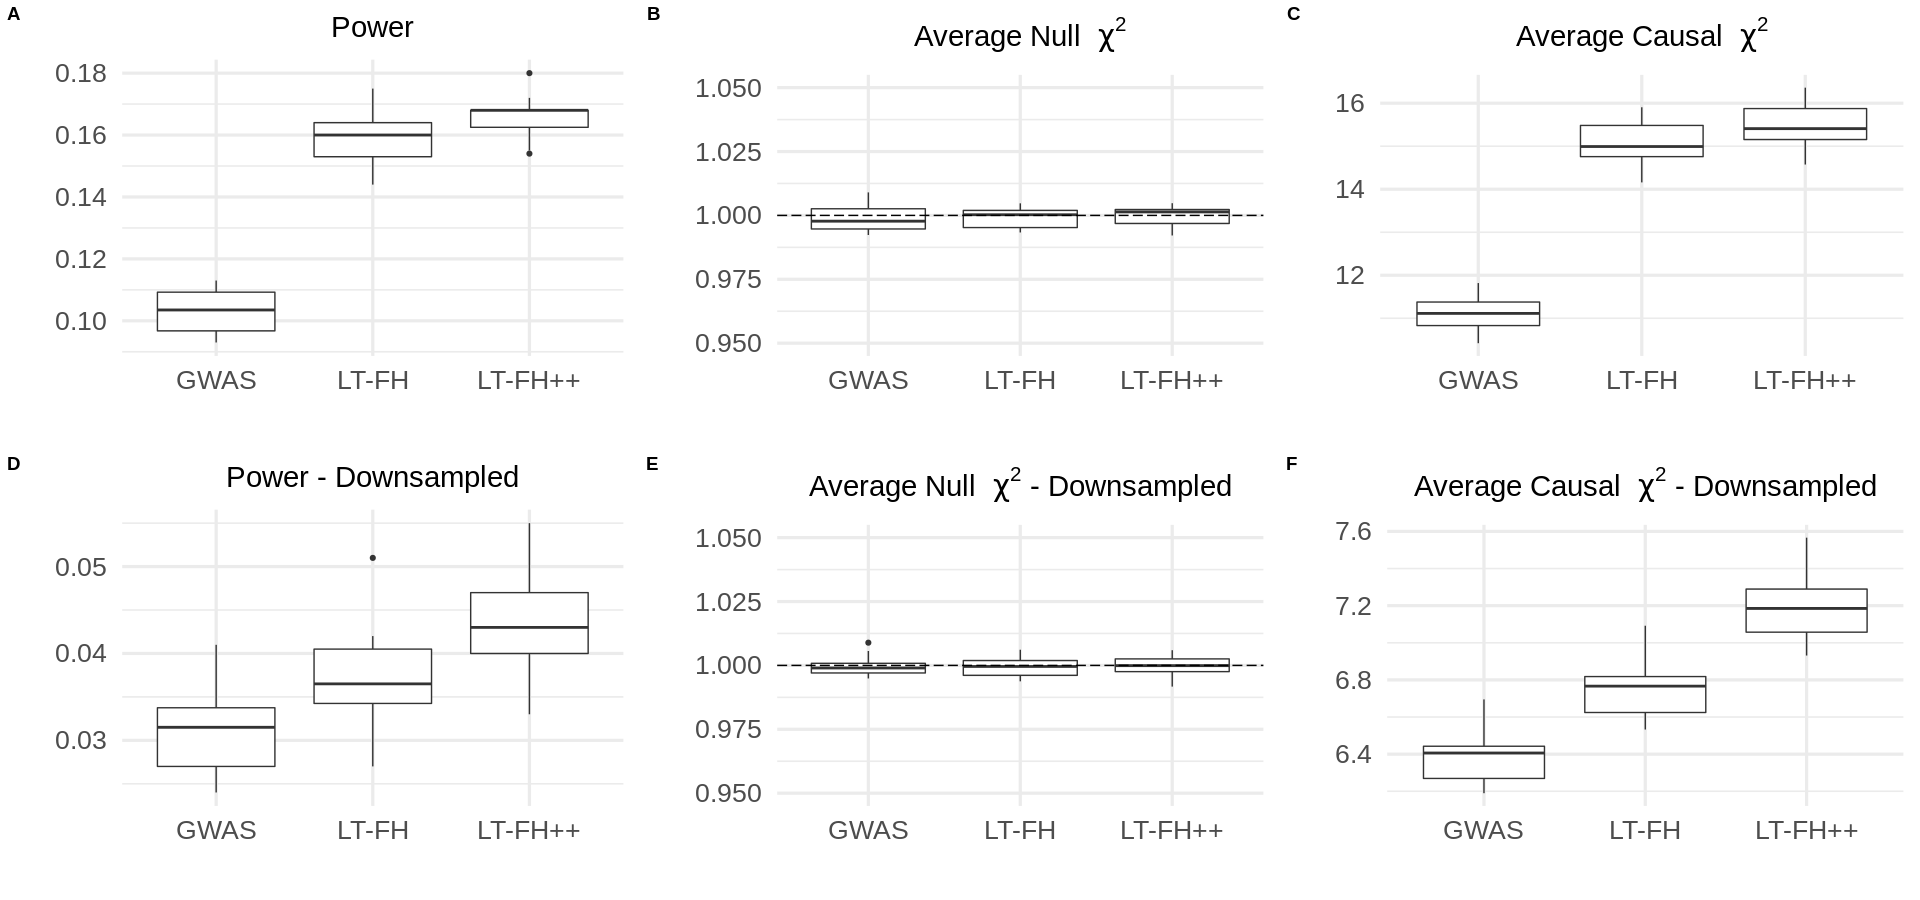
\includegraphics[width=\textwidth]{results/boxplot_05prev_both.png}
	\caption[Simulation results for a $ 5\% $ prevalence, with and without downsampling of controls]{Linear regression was used to perform the GWAS for LT-FH and LT-FH++, while a 1-df chi-squared test was used for case-control status. We assessed the power of each method by considering the fraction of causal SNPs with a p-value below $ 5 \times 10^{-8} $. Here, GWAS refers to case-control status and LT-FH and LT-FH++ are both without siblings. Downsampling refers to downsampling the controls such that we have the same number of cases and controls, i.e.\, we have $ 10,000 $ individuals in total for a $ 5\% $ prevalence and $ 20,000 $ individuals for a $ 10\% $ prevalence.}
	\label{fig:LTFHppSimulationResults}
\end{figure}

The simulations show a modest increase in favour of LT-FH++ over LT-FH in the full sample, with an average power increase across the $ 10 $ simulations of $ 4\% $. Both LT-FH and LT-FH++ has an average power increase of more than $ 50\% $ compared to the case-control status used in \textit{GWAS}, making either method vastly better. However, case ascertainment has a significant impact on the power ratio between LT-FH and LT-FH++. When case ascertainment is present in a biobank, the average power increase of LT-FH++ over LT-FH increased to $ 18\% $.

\newpage

\subsection{Real-world analysis}
\begin{wrapfigure}{O}{10cm}
	%	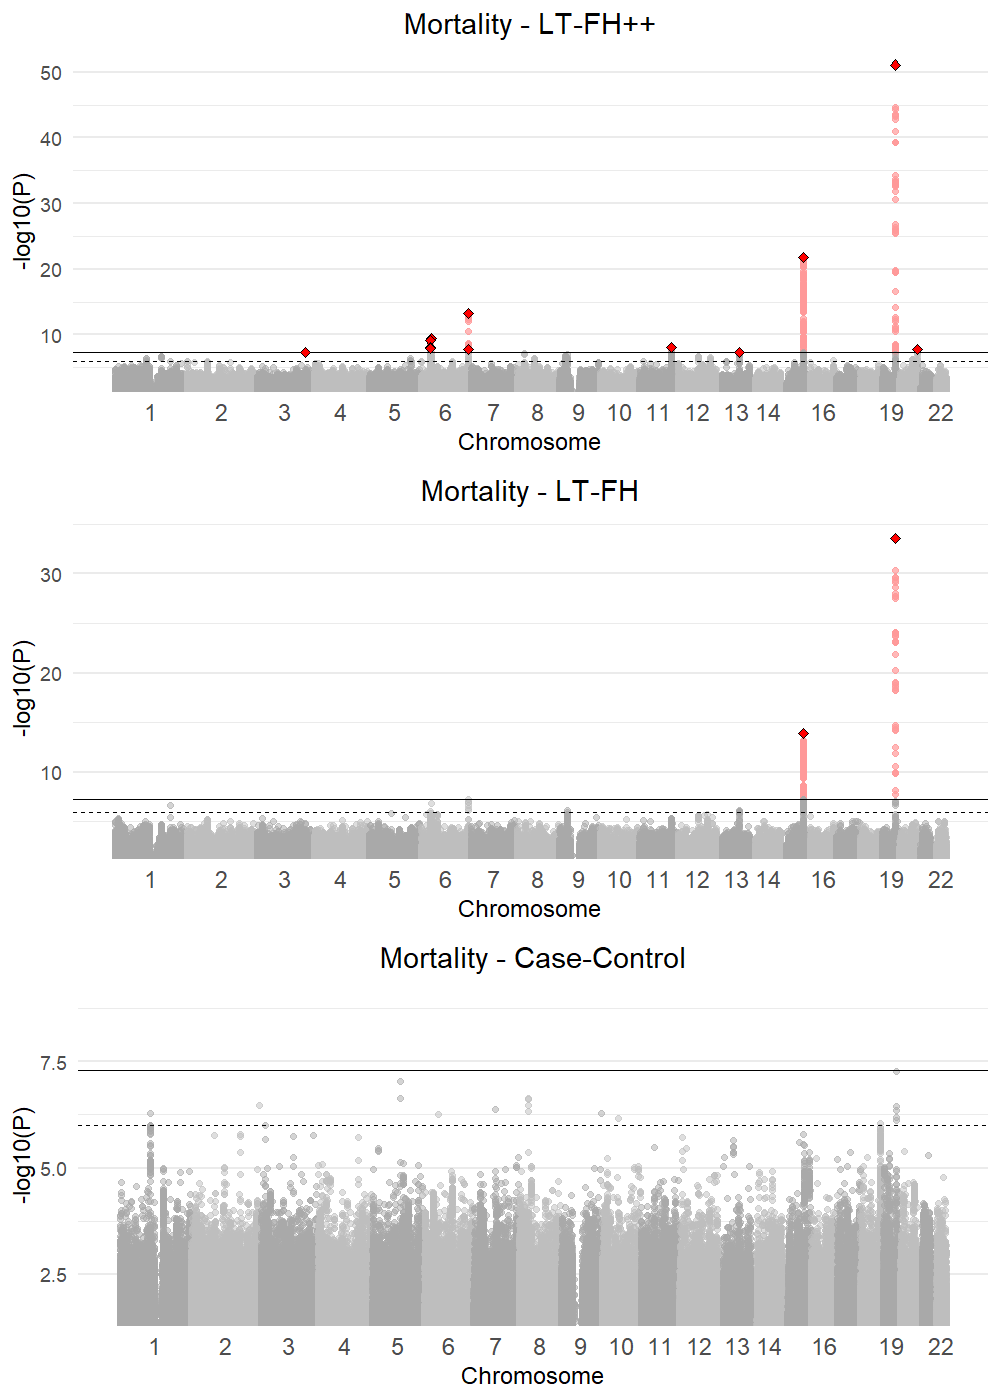
\includegraphics[width=0.7\textwidth]{results/manhattanPlot_mortality.pdf} % adds a lot of loading 
	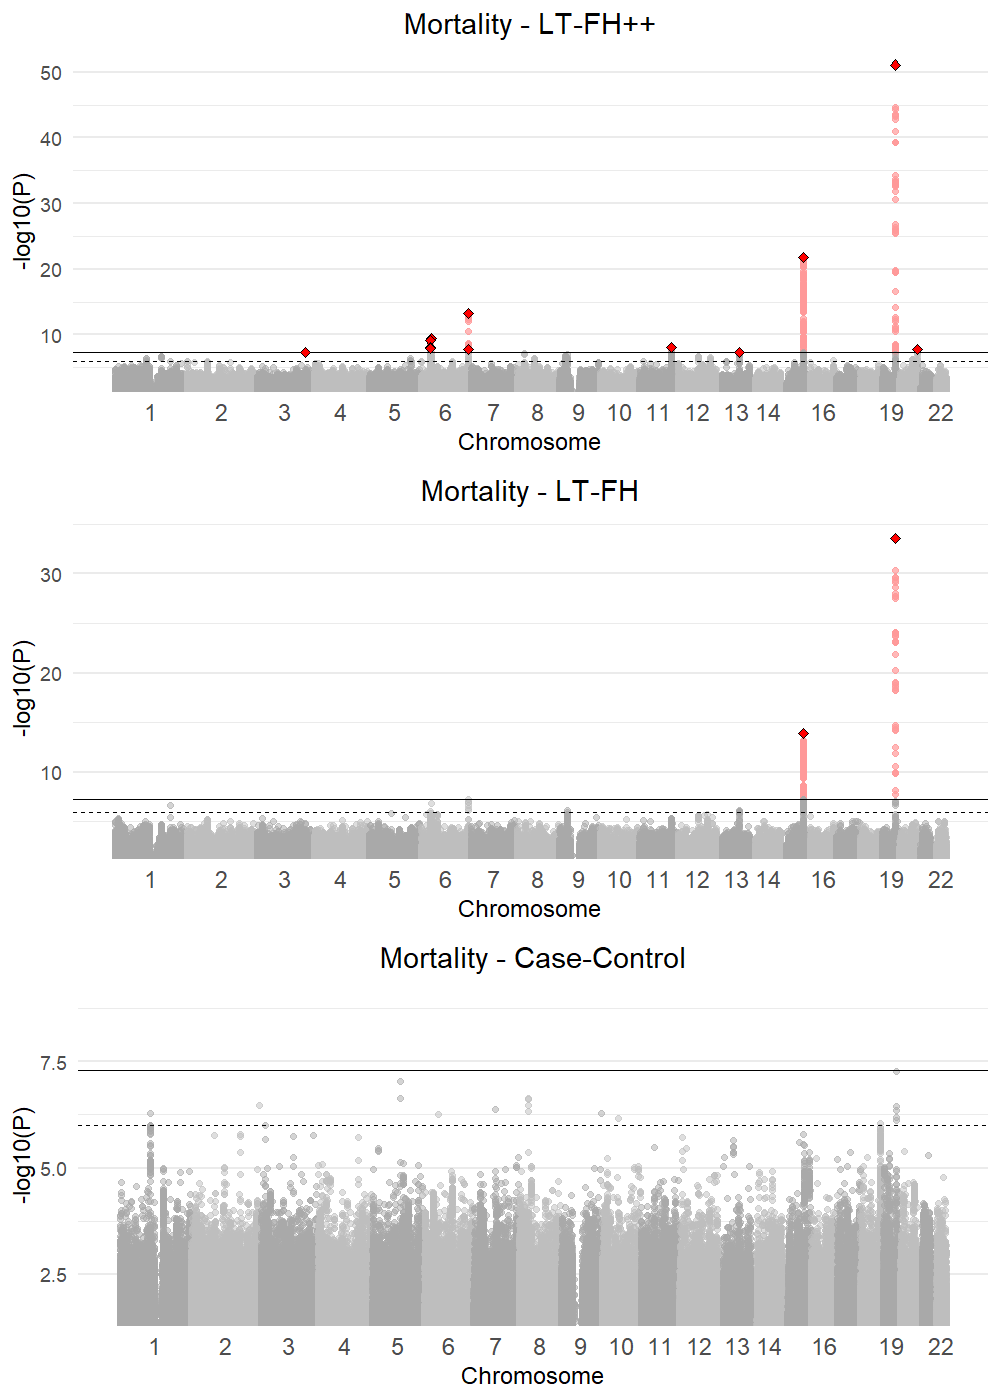
\includegraphics[width=10cm]{results/manhattanPlot_mortality.png}
	\caption[Manhattan plots for LT-FH++, LT-FH, and case-control GWAS of mortality	in the UK Biobank]{The Manhattan plots display a Bonferroni corrected significance level of $ 5\times 10^{-8} $ and a suggestive threshold of $ 5\times 10^{-6} $. The genome-wide significant SNPs are coloured in red. The diamonds correspond to top	SNPs in a window of size $ 300,000 $ base pairs.}
	\label{fig:LTFH++_manhattanMortality}
\end{wrapfigure}

LT-FH++ was also applied to four of the main psychiatric disorders in iPSYCH and to mortality in UKBB. The mortality GWAS in UKBB resulted in $ 0 $ genome-wide significant SNP for simple linear regression, $ 2 $ for LT-FH, and $ 10 $ for LT-FH++. The Manhattan plot for mortality can be found in \cref{fig:LTFH++_manhattanMortality}.

The GWAS in iPSYCH did not provide nearly as large of an increase in power for LT-FH++ or LT-FH over simple linear regression. In fact, we did not see any notable improvement over simple linear regression of the case-control status. The Manhattan plot for ADHD in iPSYCH can be found in \cref{fig:LTFH++_manhattanADHD}. We did find $ 7 $ genome-wide significant SNPs for ADHD using LT-FH++ and $ 5 $ for LT-FH and case-control status, but the two additional associations for LT-FH++ were very close to genome-wide significance for the other two outcomes as well.
\begin{wrapfigure}{R}{10cm}
	%	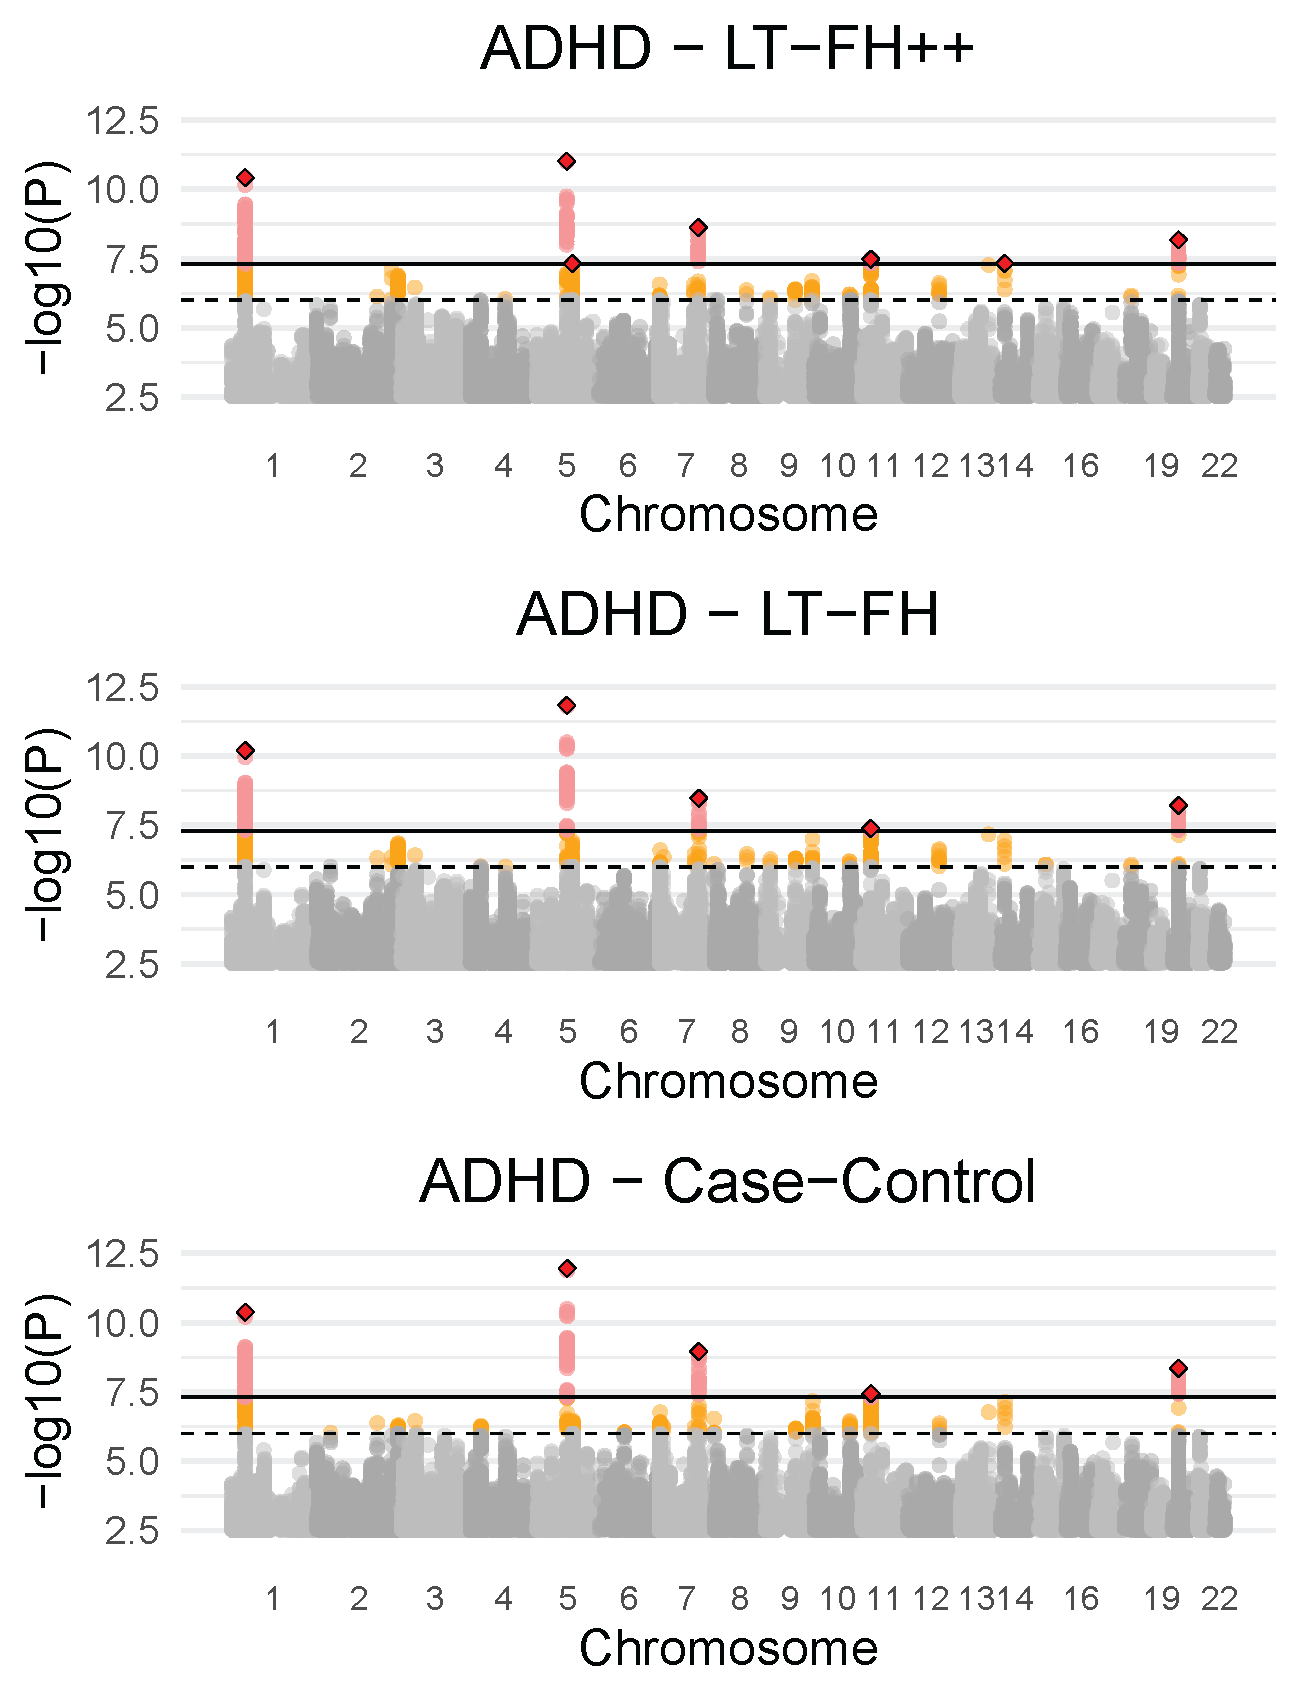
\includegraphics[width=0.7\textwidth]{results/manhattanPlot_ADHD.pdf} % adds a lot of loading 
	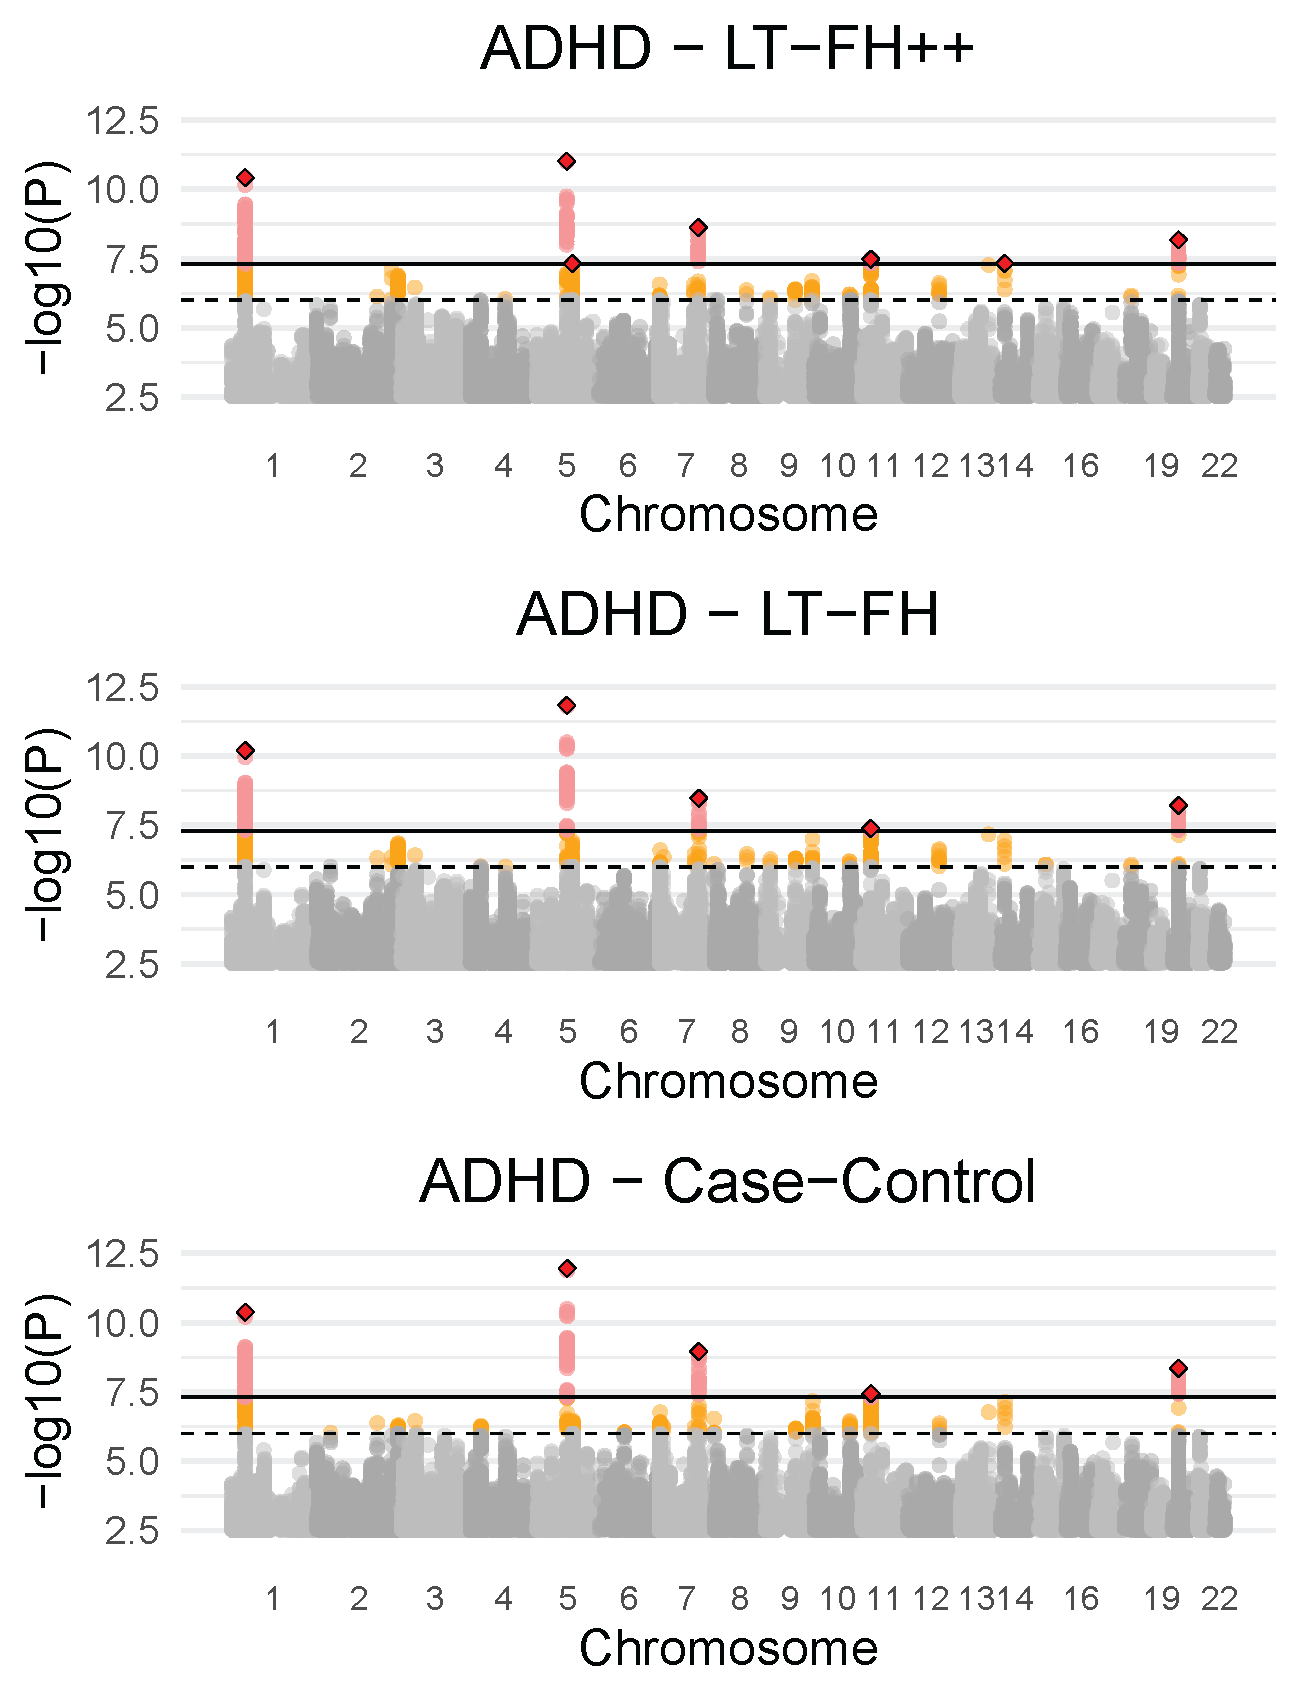
\includegraphics[width=10cm]{results/manhattanPlot_ADHD.png}
	\caption[Manhattan plots for LT-FH++, LT-FH, and case-control GWAS of ADHD in the iPSYCH data]{The dashed line indicates a suggestive p value of $ 5\times 10^{-6} $ and the fully drawn line at $ 5\times 10^{-8} $ indicates genome-wide significance threshold. The genome-wide significant SNPs are coloured in red. The diamonds correspond to top SNPs in a window of size $ 300,000 $ base pairs.}	
	\label{fig:LTFH++_manhattanADHD}
\end{wrapfigure}
Through additional simulations we found that one can expect the most \textit{relative} power gain with LT-FH++ over LT-FH if the in-sample prevalence is high in either family members or the index persons. This is because LT-FH++ is best able to utilise information for cases, since the CIPs provide a very accurate estimate for the full liability of an individual.
\newpage

\section{Paper 2 - ADuLT}
The second paper utilised the age-dependent liability threshold (ADuLT) model, which is the model underlying LT-FH++. The name change is in large part due to the focus on only the age-dependency and not family history, even though it is the same model. The purpose of the project was to examine the performance of the ADuLT outcome with established time-to-event GWAS methods that are based on the Cox proportional hazards (PH) model. It is two fundamentally different ways to approach time-to-event analysis in a GWAS setting. The adoption of Cox PH models in a GWAS setting has been limited, which has also been evident in the relative lack of method developments for Cox PH models compared to other regression models. Since one of the main limitations for Cox PH is the computational cost of such a model, GWAS with these models have been limited to less than $ 100,000 $ individuals. Recently, a method called SPACox \cite{bi2020fast} has been proposed that allows for far better scaling, and allowing for analysis of large biobanks. We will use SPACox as a representative of Cox PH models to compare to in this paper.

\subsection{Simulation results}

As for the first paper, we assessed the models in simulations first. We simulated the genotypes and assigned phenotypes with two generative models. The first model was the liability threshold model and the second model was the proportional hazards model. Notably, one would expect a method based on the liability threshold model to perform the best under this model, and subpar under other generative models. The simulation results shown in \cref{fig:adult_simulations} show the power for $ 10 $ replications under two different generative models and for different population prevalences. In \cref{fig:adult_simulations}A, the ADuLT or case-control status methods perform slightly better than the Cox PH model under the liability threshold model and vice versa, which is what we expected. Notably, there is no case ascertainment in those simulations. The results shown in \cref{fig:adult_simulations}B are with case ascertainment and we observe a large shift in power between methods under both generative models. In short, the simulation results show that the Cox PH based method has a far lower power than the LTM based methods under \textit{both} generative models, when cases are ascertained. Even after performing inverse probability weighing Cox PH on a select subset of null SNPs and all causal SNPs, we observed the same result. This indicates that the Cox PH models with the current implementation suffers from a significant power loss when case ascertainment is present in a GWAS setting, which is very common in practice.

%\begin{wrapfigure}{O}{10cm}
\begin{figure}[h]
	\centering
	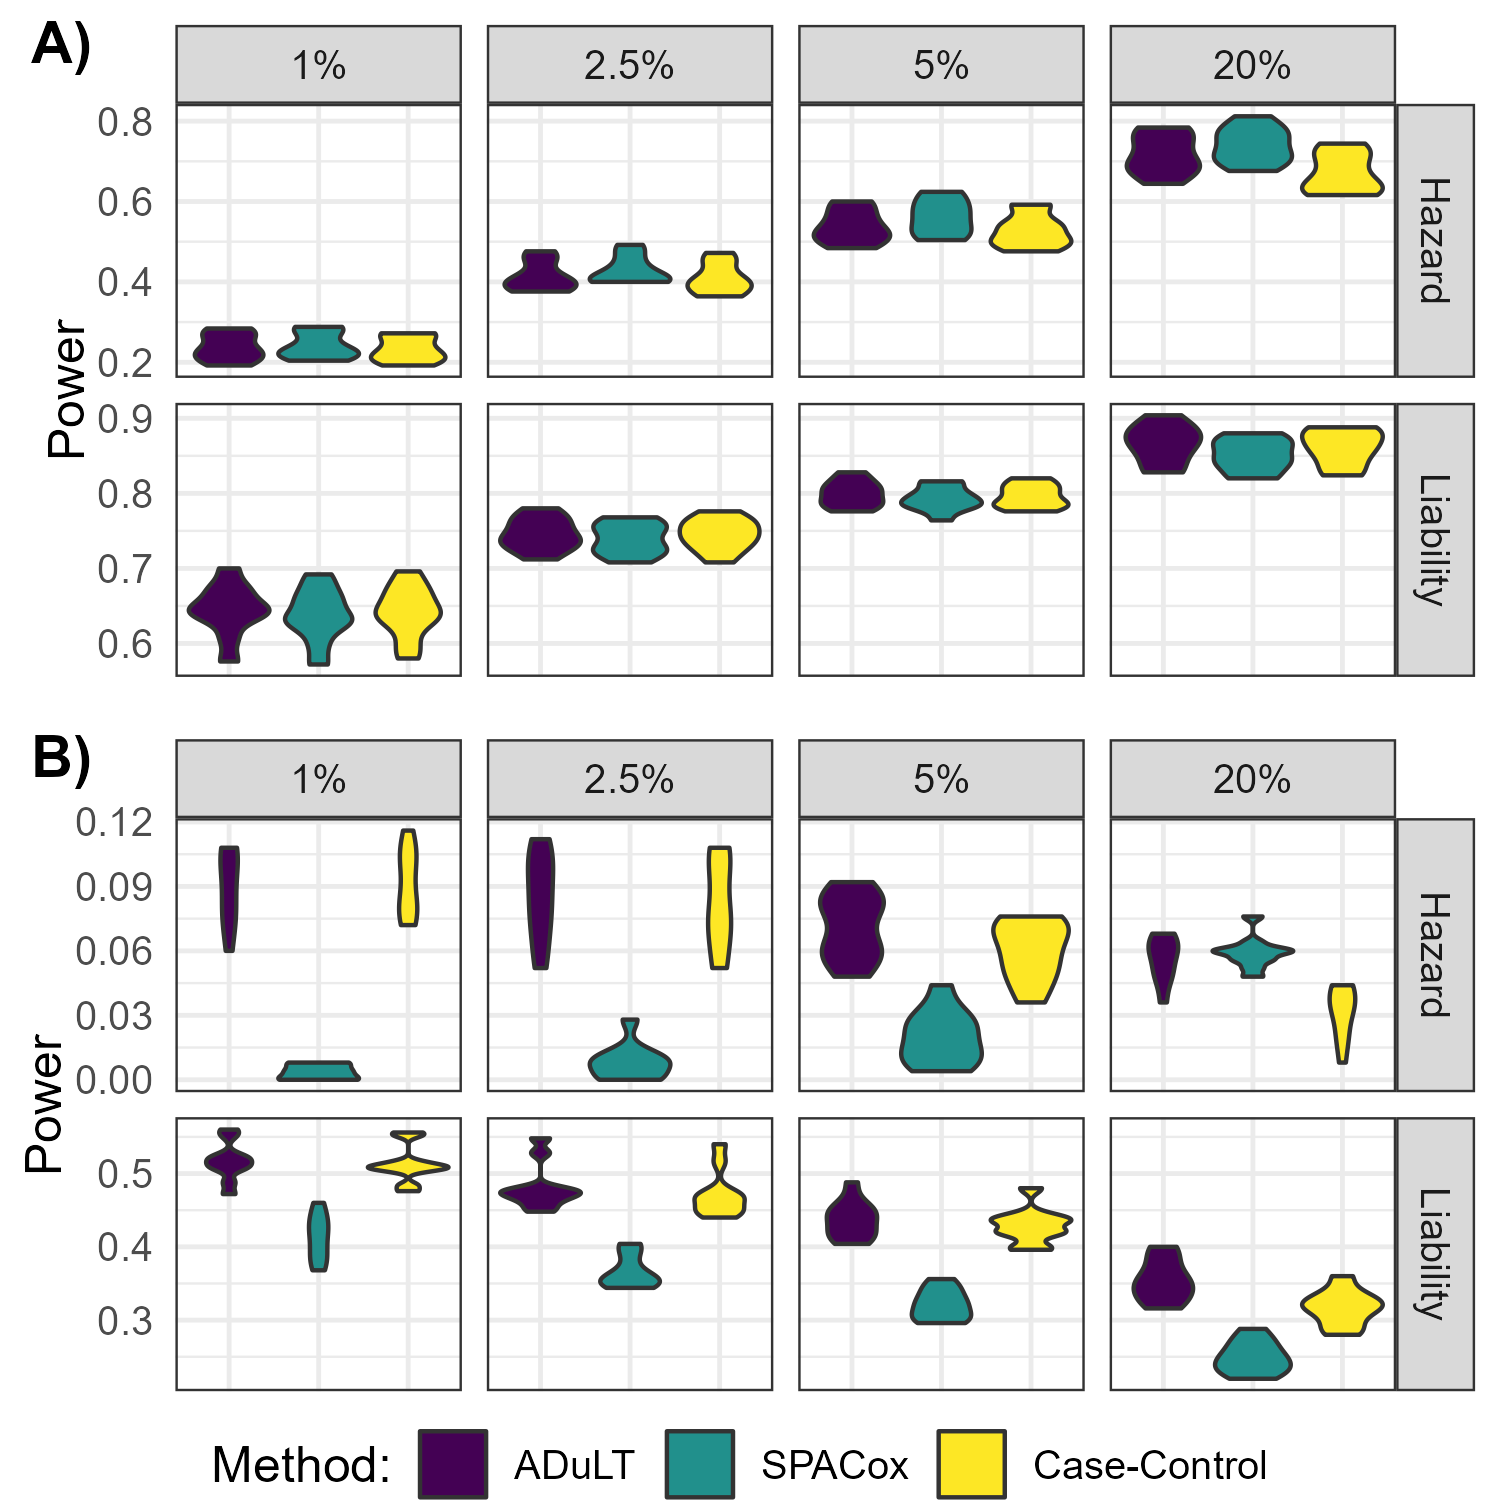
\includegraphics[width=10cm]{results/adult_combined_C250_power}
	\caption[Power simulation results with $ 250 $ causal SNPs under both generative models and varying prevalences.]{The power is shown for different population prevalence, varying from $ 1\% $ to $ 20\% $. \textbf{A)} The power, i.e.\ the fraction of causal SNPs detected for each method, \textbf{without downsampling}. \textbf{B)} The power \textbf{with downsampling}, i.e.\ the number of individuals is subsampled to 10k cases and 10k controls.}
	\label{fig:adult_simulations}
%\end{wrapfigure}
\end{figure}


\subsection{Real-world analysis}
Next, we applied the same analysis to real-world data to assess whether we observed the same behaviour with case ascertainment present in the data. iPSYCH is particularly useful for this, as all cases in a given time period have been sampled and sequenced, meaning the iPSYCH data has a high case ascertainment.

We found that the Cox PH model had a rather large loss of power compared to ADuLT and case-control status. Across the four analysed psychiatric disorders, ADuLT found $ 20 $ independent associations, case-control status found $ 17 $, and SPACox found $ 8 $. The ADHD Manhattan plots for the three methods compared in paper 2 can be found in \cref{fig:adult_ADHD}. In no circumstances did the Cox PH model outperform a LTM based method, showing that the currently implementation of Cox PH model does not perform as well as simpler models such as linear regression, which are also far more computationally efficient.

%\begin{wrapfigure}{O}{10cm}
\begin{figure}[h] 
	\centering
	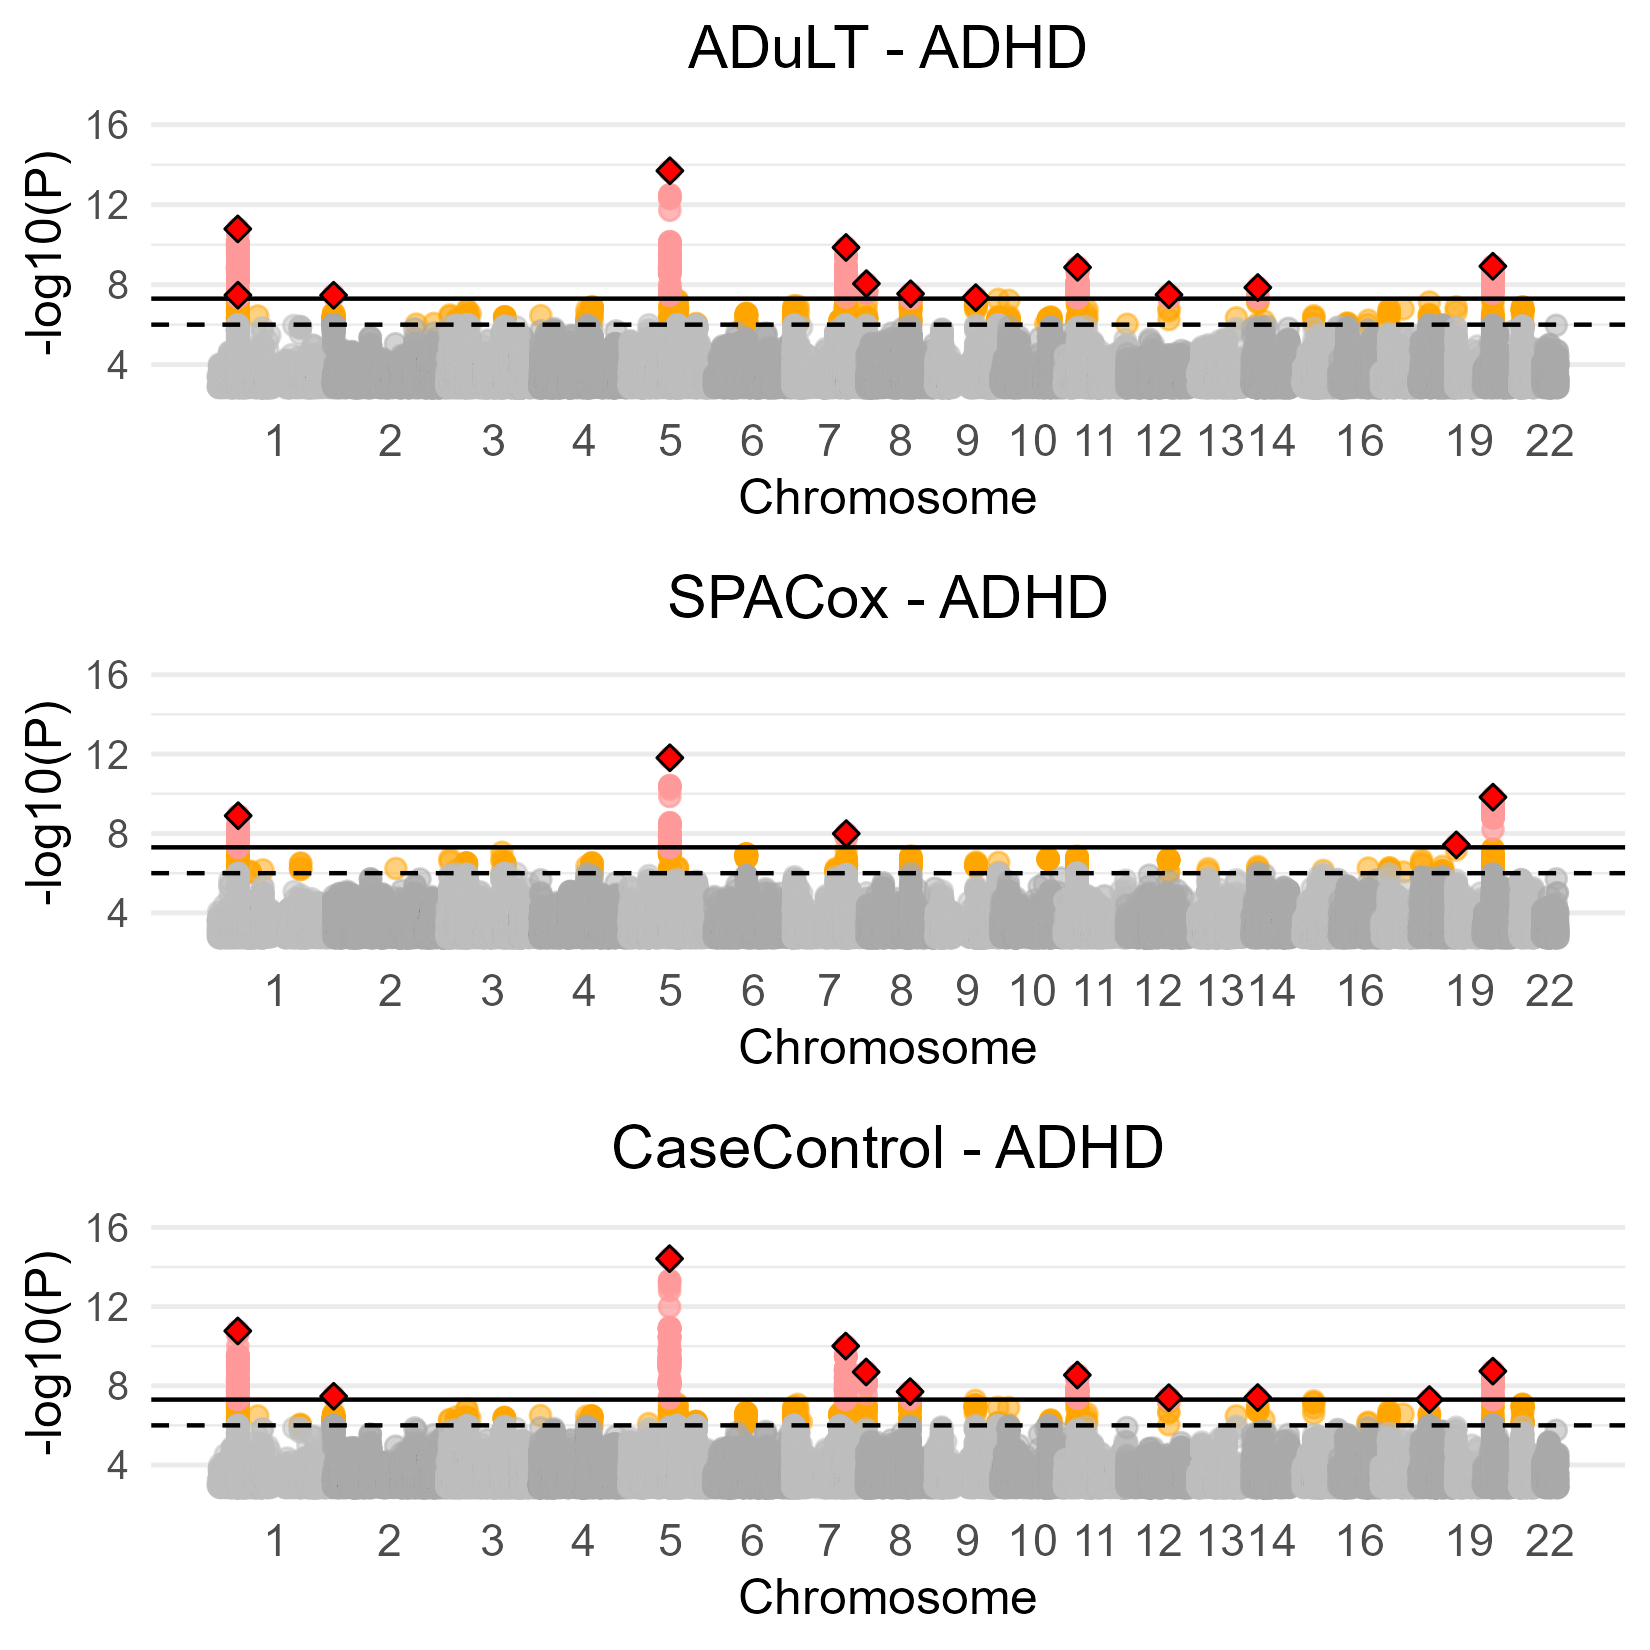
\includegraphics[width=10cm]{results/adult_manhattanPlot_ADHD}
	\caption[Manhattan plots from GWAS with the ADuLT phenotype, SPACox, and case-control status for ADHD]{Manhattan plots for ADHD for all three methods. Case-control GWAS uses the age of individuals as a covariate, whereas the ADuLT GWAS and SPACox do not. The orange dots indicate suggestive SNPs with a p-value threshold of $ 5 \times 10^{-6} $. The red dots correspond to genome-wide significant SNPs with a p-value threshold of $ 5 \times 10^{-8} $. The diamonds correspond to the lowest p-value LD clumped SNP in a 500k base pair window with an $ r^2 = 0.1 $ threshold.}
	\label{fig:adult_ADHD}
%\end{wrapfigure}
\end{figure}


\newpage

\section{Paper 3 - fGRS}
TBA
%\input{results/}


\chapter{Discussion}

\section{Paper 1 - LT-FH++}
ltfh++ discussion goes here

\begin{enumerate}
	\item more EHR means we need a better way to include that information. LT-FH++ does this for FH and AOO.
	\item most power gain when in-sample prevalence is high or when fh prev is high for the sample
	\item can easily handle missing information
	\item CIP and FH are not currently common to include
	\item CIPs can be estimated in a similar external population and used with the internal population.
	\item UKBB and iPSYCH result summary
	\item discussion reasons for why the performance is different between UKBB an iPSYCH
	\item LT-FH++'s relationship to survival analysis?
	\item LT-FH++ combines two different types of model
\end{enumerate}


Few places in the world have as detailed, curated, and complete register information linked to genetic data as iPSYCH does. Recently, there have been a trend where biobanks such as UK biobank, DeCODE, and FinnGen have started linking to registers or supplement their genetic data with questionnaires. As a result, we strongly believe that the information stored in this supplementary information can be leveraged to increase statistical power to identify causal SNPs in a GWAS setting. Family history has previously been used to generate risk scores[REF e.g. FRAMINGHAM] or been included as a covariate in epidemiological analysis[ASK ESBEN FOR EXAMPLES], and as such, is a parameter many researchers are familiar with and know its potential. Similarly, an entire branch of statistics is focused on modelling time-to-event, which means many researchers are also familiar with age of onset and recognise its potential. Here, we proposed LT-FH++ as a way to combine family history and age of onset distributions with the ordinary case-control status to increase power, thereby combining two previously separated types of analysis.

Simulations show that LT-FH++ does increase statistical power in a GWAS setting over LT-FH and case-control status. The exact power increase provided by LT-FH++ over LT-FH depends on the situation the method is applied to and varies from roughly $ 4\% $ to $ 18\% $. Through supplemental simulations we found that one can expect the highest increase in power with LT-FH++ compared to LT-FH, when cases are ascertained in the sample or in the sample's family members. The supplemental simulations have also provided valuable insight into the power difference in the real-world data analysis of UKBB and iPSYCH.

The mortality GWAS in UKBB highlights a near perfect example of LT-FH++'s potential. Death is the only guarantee in life, unlike many disorders that can be quite rare. The UKBB participants were between $ 40 $ to $ 69 $ years old at recruitment. This means many of the participant's parents have already passed or are close to their life expectancy and that the participants themselves are getting close to it. Therefore, death is prevalent among the parents and has an ever-increasing prevalence among the participants. Death has a modest prevalence in the participants, but a high prevalence among the parents. In summary, death satisfy both of the criteria for best case scenario for LT-FH++ that we identified from the simulations. 

In iPSYCH, the conditions for both LT-FH and LT-FH++ are not nearly as favourable. The largest source of power increase provided by LT-FH and LT-FH++ are from the family history information. LT-FH++ further refines this information with the age of onset distributions, but as simulations show, it provides up to $ 18\% $. Due to psychiatric disorders such as ADHD not being present in ICD-8, it limits the opportunity to diagnose many of the parents of the iPSYCH participants. This is true even though the iPSYCH participants are much younger than the UKBB participants. The design of iPSYCH also means that most affected siblings have already been selected, sequenced, and are themselves present in the data. In summary, the family history seem to be lower than expected, due to the family either being sampled themselves or being too old to be easily diagnosed. However, even if an affected sibling pair is present and filtering would exclude one sibling, their status would still increase the liability of the remaining sibling, which would not be the case for case-control status.

The polygenicity of the analysed phenotypes are also likely to be different. Death can numerous sources, such as cancer, heart diseases, or accidents. Accidents are not likely to have a genetic signal, while cancers, heart diseases, smoking, etc. are. Some cancers and heart disease have one or more prominent genetic signals \textbf{FIND SOME EXAMPLES WHERE THERE IS A LARGE PEAK, E.G APOE ?}. On the other hand, psychiatric disorders have proven to be very polygenic, meaning there are many SNPs with a small effect size. This coupled with the relatively smaller sample size of iPSYCH compared to UKBB, may mean identifying genome-wide significant associations are harder.

Both LT-FH and LT-FH++ require additional information to estimate the underlying genetic liabilities. The availability of family history is still limited in practice for most biobanks, which limits their applicability. Unfortunately, the family history information cannot be acquired by means other than registers, questionnaires, etc. The same is not necessarily true for the CIPs. In sample, information such as birth year, age-of-onset, and sex are often available to some extent. For instance, the age of onset may be slightly anonymised, such that the exact day or month may not be available, but a reasonable approximation is still known. The CIPs used by LT-FH++ are population representative and summarise the age-specific proportion of the considered phenotype. This means they can be used in different populations, as long as the populations are similar. As an example, CIPs derived from the Danish registers could be used with, e.g. other Scandinavian countries or the UK. As there are differences in diagnostic practices across countries, some care should be taken when using CIPs for other populations. For instance, if the CIPs are based on psychiatrists and the disorder of interest in a biobank is self reported. When using the CIPs in a different population, we would not recommend fixing the thresholds for cases, but rather let the lower limit be determined by the CIP and the upper limit be infinite. 

\section{Paper 2 - ADuLT}
adult discussion goes here


The purpose of this paper was to examine the best way to include the age of onset information in a GWAS setting. The gold standard when modelling time to event is some kind of survival analysis. However the adoption of such methods such as Cox regression have been limited for GWAS. One of the main limiting factors for Cox regressions, such as the proportional hazards model, is the computational cost associated with the analysis. Recent advances have allowed for Cox proportional hazards models and frailty models to be used on UKBB-sized biobanks. Both methods utilise a saddle point approximation, as it provides a computationally efficient way to calculate p values. The implementation of the proportional hazards model is called SPACox and is available as an R package. The frailty model has been implemented in a R and Rcpp, which is a R-wrapper around C++. 




\section{Paper 3 - Family Liabilities}
The use of family history as a predictor of disease risk has long been a subject of interest in epidemiology and preventive medicine. While family history captures both environmental and genetic variation, including the so-called "missing heritability", its predictive power is often limited by the use of binary indicators to account for the presence or absence of a particular disorder in the family. 

In this study, we repurposed to utilise the LT-FH++ model to quantify individual family history risk and estimate individual family liabilities (FL). This means estimating the liability of the index person, but ignoring the disease status in the individual, such that all information is derived from the family members. It is similar to the previously proposed family genetic risk scores by Kendler et al.\cite{kendler2021family} and the FL estimated under the LT-FH++ model is a time-to-event model that accounts for differences in prevalences by birth year and sex, as well as accounting for age. By using a model-based approach, we aim to improve the interpretability and predictive power of family history as a risk factor, as the Kendler et al. is a heuristic approach. We evaluate the performance of our method using data from the Danish registers and iPSYCH study, and compare it to binary family history indicators, as well as PRS. Our results show that FL estimates have improved predictive accuracy over standard binary family history indicators. We note that this result is in stark contrast to previous results by Hujoel et al.\cite{hujoel2022incorporating}, which found that estimating family risk using a multivariate liability threshold model provided little or no benefit over binary family history indicators. However, we believe this is due to both more detailed family history information available in the Danish registers (parents, siblings, children, paternal and maternal half-siblings and grandparents), as well as our proposed model accounts for sex, birth year, and age or age-of-onset for all family members. 

We further proposed combining FLs for multiple correlated health outcomes to improve their predictive accuracy. We found this approach to provide less benefit over the comparable approach of combining family history indicators for multiple correlated health outcomes. While the predictive accuracy of the extension to genetically correlated health outcomes was not improved, it still has potential as an accurate liability outcome in a GWAS. As the multi-trait extension estimates a single value, this application is of particular interest and an area of future research.
Similar to previous work\cite{mars2022systematic,wolford2021utility,hujoel2022incorporating}, we found that PRS and family risk measures captured largely independent information. We note that there are several reasons for this independence between PRS and FL. First, the accuracy of the PRS is limited by heritability explained by the genotyped variants, whereas FL can (in theory) capture any additive genetic variance (full heritability) as well as shared environmental effects. Second, FL and PRS are trained on different data, with PRS using external summary statistics and genotypes and FL using register information. Third, given current sample sizes, their absolute variance explained is small which makes it unlikely that they capture the \enquote{same} variance. 

There are several limitations to our study, some of which we aim to address in future or ongoing research. First, both the Binary family history and the FL variables are subject to limitations on available family history in biobanks or registers. If no or only limited family history information is available, these methods are unlikely to provide a significant increase in prediction accuracy. For example, UKBB only has family history available for $ 12 $ phenotypes, with full family history information only available for parents. Second, the predictive accuracy of FL is unlikely to have unbounded potential for improvement as more family information becomes available, as families are rarely very large and are not likely to increase substantially in the future. However, our work suggests that combining family history for multiple outcomes may further improve FL. Third, the model underlying FL assumes that the full additive (narrow sense) heritabilities and genetic correlations are known. However, these may not always be available, nor be easily estimated in the family data. We aim to address this limitation by estimating these parameters directly from the family data. Finally, using the average PC value as a reference when calculating the genetic distances used to stratify prediction accuracies could be a poor reference choice, as it may not match individuals of Danish genetic ancestry well. We aim to remedy this by using a more precise Danish genetic ancestry reference using a similar approach as Privé et al.\cite{prive2022portability}.

While family history is still not widely available in biobanks, an ever-increasing number of biobanks have some level of family history information, and this trend is likely to continue. The biobanks that already have family history information may continue to expand on them, further increasing their utility. As illustrated by the multi-trait analysis performed here, utilising correlated phenotypes, either through family history or PRS, has a significant potential to improve overall prediction of a particular phenotype. Combining FLs and PRS has the potential to increase prediction even further, as they conceptually estimate the same thing, while being largely independent.



\chapter{Conclusion}
The dissertation has focused on the development, implementation, and application of what is now called LT-FH++. LT-FH++ extends the previously published LT-FH method, which is itself an extension of the classical liability threshold model by Falconer. LT-FH extended the LTM such that it models family members for binary traits, which allowed for an estimate of a genetic liability that, when used as the outcome in a GWAS, provided a significant power increase. LT-FH++ extensions this framework even further by also accounting for age of onset in cases or age in controls, sex, and birth year. These things are accounted for through population representative cumulative incidence proportions that are stratified by sex and birth year. This leads to a threshold in the LTM that is unique for each individual, which has not previously been done. Since every individual has a unique threshold, a more computationally efficient sampling strategy had to be implemented than what was used in LT-FH. As a result, LT-FH++ utilises a Gibbs sampler that samples from a truncated multivariate normal distribution that allows for arbitrary thresholds. Furthermore, the implementation is parallelizable, which allows it to better utilise modern CPUs with many cores or high performance computing clusters.

In the first project, most of the code base and methodological development work was done. It culminated in the publication of the LT-FH++ method, which refined a liability that was informed by family history \textit{and} age of onset, sex, and birth year for each included individual. LT-FH++ performed between $ 4\% $ and $ 18\% $ better than LT-FH in terms of identifying the true causal associations in a simulated GWAS setup. Both LT-FH and LT-FH++ outperformed the conventional case-control status and the GWAX phenotype. For a real-world analysis, mortality in the UKBB was analysed and four psychiatric disorders from iPSYCH. For mortality, LT-FH++ significantly boosted power compared to LT-FH and case-control status. LT-FH++ was able to identify $ 10 $ genome-wide significant SNPs, while LT-FH identified $ 2 $ and case-control status identified $ 0 $. In iPSYCH, the difference between the three phenotypes was modest. There are likely several reasons for the lack of power gain over case-control status by LT-FH and LT-FH++, such as low family history prevalence and more polygenic disorders. Additional simulation studies also revealed that the mortality setup in UKBB was a near perfect scenario for LT-FH++, since it benefits from a high prevalence in either the genotyped individuals or in the family history.

The second project examined the best way to include age of onset in a GWAS setting. This meant comparing the model underlying LT-FH++, here called ADuLT as no family history was used, to other time-to-event GWAS methods. The simplest and most commonly used time-to-event GWAS method is the Cox proportional hazards model. Since the Cox proportional hazards models are computationally intensive most implementations are unable to handle more than $ 100,000 $ individuals, and we will use the most computationally efficient implementation called SPACox to represent these models. We will compare the performance of ADuLT, SPACox, and case-control status in a linear regression. We simulated genotypes and assigned phenotypes and age of onset under both the proportional hazards model and the LTM. One would expect the LTM models to perform the best when phenotypes were assigned with the LTM, and vice versa, which is also what we observed. However, when we emulated case ascertainment, meaning we downsampled the controls such that we had an equal number of cases and controls, we observed a disproportionate loss in power for SPACox. Conventionally, IPW would be used to account for the ascertainment, however it had no effect here and SPACox still performed worse than simple linear regression, even under the proportional hazards model. The same disproportionate loss of power was also observed in real-world analysis of iPSYCH disorders. As a result, we do not recommend proportional hazards to identify genome-wide significant SNPs, instead a simpler linear regression or ADuLT in a GWAS method of choice should be used.

The third and final project examined the predictive value of family history. Normally, a binary family history variable is used, such that an affirmative value is given to individuals with at least one case in their considered family, e.g.\ first degree relatives. This was compared with the PRS of the considered phenotype, as well as the LT-FH++ phenotype without any information on the index individuals. This means the LT-FH++ estimates the genetic liability solely based on the family history. We assessed the predictive value with the partial $ R^2 $ in a regression model. A base model was used with age, sex, and the first $ 20 $ PCs. Then a model with either of the family history phenotypes was considered, a model with the PRS, and a model with any combination of these. In short, LT-FH++ had an increased partial $ R^2 $ compared to the PRS model of $ 19.6\% $ across the $ 8 $ considered disorders. The binary family history variable had a $ 65.2\% $ \textit{decrease} compared to the PRS model. The model with both the binary family history variable and the LT-FH++ phenotype had almost the same predictive value as the model with only the LT-FH++ phenotype. Interestingly, the model with the LT-FH++ phenotype and the PRS had an almost additive increase in their predictive value, indicating that they capture independent genetic signals. The model with all three predictors performed nearly identically to the model with just the LT-FH++ phenotype and the PRS, indicating that all signal is captured by those predictors. 
 
As most psychiatric disorders have a high genetic correlation, we also considered a regression model that included correlated phenotypes in the prediction model. The average of these phenotypes were higher than their single trait equivalent, but difference between LT-FH++ and the binary family history variable had largely disappeared, making both variables equally predictive. The model with both family history phenotypes was had nearly the same predictive power as either of the family history models, meaning no new information was gained by using both. Combining the multi trait PRS model with either of the family history phenotypes resulted in a model with close to the sum of the PRS and family history model's predictive values. This means that even for correlated phenotypes, the genetic signal captured by the PRS and the family history phenotypes appear to be nearly independent.

In summary, we have successfully developed, implemented, and applied the LT-FH++ method in a number of different areas. The LT-FH++ method has provided improvements in each of the three applications that have been considered, while remaining computationally efficient. While family history and age of onset is not commonplace in all biobanks yet, we have demonstrated that it is a worthwhile investment, as power to detect associations in a GWAS setting, with or without family history, and the predictive value of family history have been increased by using the LT-FH++ phenotype instead of the binary variables that are commonly used.



\chapter{Future directions}
During the dissertation, we have illustrated that the LT-FH++ phenotype has increased power in GWAS, outperformed standard survival GWAS methods when case ascertainment is present, and improved the predictive value of family history. LT-FH++ has managed to provide a computationally efficient link between the liability threshold model and survival models that can account for concepts such as censoring and family history. To the best of our knowledge, this link is a novel one that has not been examined or developed much yet. As a result, the first potential direction for future research is to examine this connection in greater detail, such that it will be possible to better understand how LT-FH++ fits in the existing survival analysis literature.

Conceptually, the genetic liability that LT-FH++ estimates share a lot of similarities with the purpose of the PRS. This relationship ought to be examined more, especially since the results from the third project of the dissertation almost showed an independent contribution from the LT-FH++ phenotype and the PRS. If they are conceptually the same, one would expect them to capture the same underlying signal, which did not seem to be the case in that project. Further examination of this relationship is therefore of particular interest. In a similar vein, if the PRS and LT-FH++ phenotype attempt to estimate the same underlying value, perhaps the PRS can be incorporated into the LT-FH++ model such that an even more accurate liability can be estimated.

Furthermore, applying LT-FH++ to new data sets is also of interest. The stay abroad during the PhD was focused on applying LT-FH++ to the FinnGen data. Unfortunately, the project was not complete during the stay, but due to time constraints in the PhD has not been completed yet. However, there are currently plans to continue this project in the future. In the Danish registers, a multi generational register is also under development, which aims to create complete family trees from $ 1930 $ and onwards, which would allow for far larger family trees than what is currently possible. LT-FH++ has already been extended to allow for more than just parents and siblings, and this multi generational register is an obvious area of application of LT-FH++. 




\chapter{English abstract}
This dissertation focuses on leveraging age-of-onset information and family history to better estimate disease liability and improve statistical power in genome-wide association studies. This is achieved through the  development, implementation, and application of a method called LT-FH++, which extends the previously published LT-FH method, and is based on the classical liability threshold model. LT-FH seeks to estimate a genetic liability based on family history, which has been shown to significantly increase power in GWAS. LT-FH++ extends this further by also accounting for age-of-onset in cases and age in controls, as well as sex, and birth year for all included individuals. This information is accounted for through population representative cumulative incidence proportions that are stratified by sex and birth year. This also allows the model to account for ascertainment biases when estimating disease liabilities. In practice, this leads to a threshold in the LTM that is unique to each individual. LT-FH++ utilises a computationally efficient Gibbs sampler that samples from a truncated multivariate normal distribution. The implementation is parallelizable and highly scalable for modern CPUs with many cores or high performance computing clusters. 

The thesis is in three parts, where each corresponds to one paper. The first part implements LT-FH++ and benchmarks it as a method for GWAS using both extensive simulations as well as UK biobank data and iPSYCH data. The second part examines the age-dependent liability threshold model (underlying LT-FH++) as a robust and computationally efficient survival analysis GWAS method, and benchmarks it against state-of-the art approaches using simulations and the iPSYCH data. The third last part focuses on using LT-FH++ for prediction based on family history liabilities for psychiatric disorders and extends the model to allow for correlated phenotypes. 


\chapter{Danish abstract}
Denne afhandling fokuserer på at udnytte familie historik og age-of-onset til at estimere en persons tilbøjelighed for en sygdom og til at forbedre statistisk styrke i GWAS. Dette opnås ved at udvikle, implementere og anvende en metode kaldet LT-FH++, som udvider den allerede udgivet LT-FH metode, som er baseret på den klassiske liability threshold model. LT-FH estimerer en genetisk tilbøjelighed til at blive syg baseret på familie historik, og det er allerede vist, at den genetiske tilbøjelighed kan forøge den statistiske styrke i GWAS. LT-FH++ udvider denne model yderligere ved også at tage højde for age-of-onset hos de sygdomsramte og alderen på kontrollerne, samt køn og fødselsår for alle inkluderet personer. Der tages højde for denne ekstra information igennem en populations repræsentativ kumulativ incidensproportion, som er stratificeret på baggrund af køn og fødselsår. Det tillader at modellen også kan tage højde for ascertainment bias når sygdomstilbøjeligheden estimeres. I praksis vil det betyde, at hver person kommer til at have en unik tærskelværdi i LTM. LT-FH++ benytter en beregningsmæssig effektiv Gibbs sampler, som sampler fra en trunkeret multivariat normalfordeling. Implementeringen kan paralleliseres og er skalerbar til at drage nytte af de mange CPU kerner, som er almindelige på moderne CPU'er, eller high performance computing clusters.

Afhandlingen består af tre dele, hvor hver del svarer til en artikel. I den første artikel blev LT-FH++ implementeret og benchmarket som en GWAS metode igennem simuleringer og anvendelse i UK biboank og iPSYCH. Den anden artikel undersøger modellen, som LT-FH++ er bygget på (age-dependent liability threshold model), som et robust og beregningsmæssig effektivt alternativ til andre state-of-the-art overlevelsesanalyse GWAS. Her benytter vi os af simuleringer og anvendelse i iPSYCH. I den tredje og sidste artikel benytter vi LT-FH++ til at estimere familie historie tilbøjeligheder for psykiatriske sygdomme og prædiktere sygdommene med disse. Vi udvider også modellen, således den er i stand til at tage højde for sigdomme. Her sammenligner vi også med en konventionel binær familie historik og PRS.





%\begin{appendices}

%\chapter{Study 1}
%study 1 goes here. \cite{pedersen2022accounting}
%\include{�}

%\chapter{Study 2}
%study 2 goes here.
%\include{�}

%\chapter{Study 3}
%study 3 goes here.
%\include{�}

%\end{appendices}

%\nocite{*}
\newpage
\printbibliography[heading=bibintoc,
title={References}]
\newpage

\end{document}